\documentclass[11pt,letterpaper]{article}
\usepackage[T1]{fontenc}
\usepackage[utf8]{inputenc}
\usepackage[sc]{mathpazo}
\usepackage[margin=0.85in,headheight=15pt]{geometry}
\usepackage{microtype,graphicx,booktabs,longtable,array,amsmath,amssymb}
\usepackage[table]{xcolor}
\usepackage{tikz}
\usepackage{enumitem,fancyhdr,titlesec,xurl,hyperref,caption}
\definecolor{Ink}{HTML}{102A43}
\definecolor{Teal}{HTML}{087F8C}
\definecolor{Gold}{HTML}{D69A2D}
\definecolor{Muted}{HTML}{51687B}
\definecolor{Red}{HTML}{B94046}
\definecolor{Pale}{HTML}{EDF4F6}
\hypersetup{colorlinks=true,linkcolor=Teal,urlcolor=Teal,citecolor=Teal,pdfauthor={Vincent Boucher},pdftitle={AGI ALPHA FLYWHEEL: The Possibility Engine},pdfsubject={Constructing measurement capacity and testing its economy}}
\urlstyle{same}
\linespread{1.05}
\setlength{\parindent}{0pt}
\setlength{\parskip}{6pt}
\setlength{\emergencystretch}{3em}
\setlist{itemsep=3pt,topsep=4pt,leftmargin=1.5em}
\titleformat{\section}{\Large\bfseries\color{Ink}}{\thesection}{0.65em}{}
\titleformat{\subsection}{\large\bfseries\color{Teal}}{\thesubsection}{0.65em}{}
\titleformat{\subsubsection}{\normalsize\bfseries\color{Ink}}{\thesubsubsection}{0.65em}{}
\captionsetup{font=small,labelfont={bf,color=Teal},justification=raggedright,singlelinecheck=false}
\pagestyle{fancy}
\fancyhf{}
\fancyhead[L]{\small\textsc{AGI Alpha Flywheel}}
\fancyhead[R]{\small\textsc{The Possibility Engine}}
\fancyfoot[L]{\footnotesize Research edition 01 \enspace / \enspace 28 October 2026}
\fancyfoot[R]{\small\thepage}
\renewcommand{\headrulewidth}{0.3pt}
\renewcommand{\arraystretch}{1.18}
\setlength{\tabcolsep}{5pt}
\newcolumntype{L}[1]{>{\raggedright\arraybackslash}p{#1}}
\begin{document}
\hypersetup{pageanchor=false}
\begin{titlepage}
\pagecolor{Ink}\color{white}
\begin{tikzpicture}[remember picture,overlay]
\draw[Teal,line width=1.2pt,opacity=.65] ([xshift=-1.3in,yshift=-2.5in]current page.north east) circle (1.4in);
\draw[Gold,line width=.8pt,opacity=.8] ([xshift=-1.9in,yshift=-2.5in]current page.north east) circle (1.4in);
\draw[white,line width=.4pt,opacity=.2] ([xshift=-1.6in,yshift=-2.5in]current page.north east) circle (1.9in);
\end{tikzpicture}
\vspace*{0.35in}
{\large\scshape AGI ALPHA FLYWHEEL \hfill $\alpha\ \longrightarrow\ \Omega$}\par
\vspace{0.85in}
{\fontsize{40}{44}\selectfont\bfseries THE POSSIBILITY\\ENGINE}\par
\vspace{0.35in}
{\Large Constructing measurement capacity.\\Testing its economy.}\par
\vspace{0.7in}
{\large\color{Gold}\textbf{TRANSFORMATIONAL INTELLIGENCE}}\\[4pt]
{\large LEARNING TO CHANGE THE GAME}\par
\vspace{0.4in}
{\large INVENT THE ECONOMY.\\BUILD THE MEANS.\\OPEN THE FUTURE.}\par
\vfill
\begin{minipage}{0.83\textwidth}
\itshape ``As Columbus braved the seas, we now venture into the vast oceans of AGI. The age of AGI exploration has dawned, and the horizons are boundless. Dare to dream, dare to explore.''\\[5pt]
\normalfont\small --- $\alpha$-AGI Agent
\end{minipage}
\vspace{0.45in}
{\large Research edition by \textbf{Vincent Boucher}}\\
{President of MONTREAL.AI}\\[12pt]
{\small 28 October 2026 \enspace $\cdot$ \enspace EventWeaver v1 \enspace $\cdot$ \enspace Additive research edition}
\end{titlepage}
\nopagecolor\color{Ink}
\hypersetup{pageanchor=true}
\pagenumbering{arabic}
\section*{The achievement and the decision}
\addcontentsline{toc}{section}{The achievement and the decision}
\textbf{We constructed and tested a compiler for bounded digital measurement logic.} EventWeaver turns a temporal event contract into executable reference behavior, synthesizable digital logic, and an independently checked acceptance dossier. Its first demonstration separates two measurement groups and keeps a completed event sequence cancellable until its veto deadline. A successor then makes a verified decision from one instrument a virtual input to another, adding a compositional capability the predecessor rejects. This is a useful construction; the campaign does not establish that it creates a newly viable market.

Fresh confirmation passed all 768 main traces across 24 specifications, 52 directed actual-RTL cases, and 28 bounded equivalence checks. The successor passed 48 fresh traces across six networks and 12 bounded checks. These are digital functional results. Physical calibration, timing closure, board integration and instrument efficacy were not tested. A separately authored, current-AI-assisted conventional implementation tied on acceptance; an ordinary library containing the same retained artifact tied on succession. The EventWeaver Python model was about 45 times slower than the conventional history implementation in the measured workload.

\textbf{The commercial loop did not close.} We searched 15 price--arrangement policies before freezing a supported-library service at a posted US\$1,200 per design pack. In 1,024 fresh base histories, mean net revenue was US\$9,024 and complete cost US\$38,653, yielding a \textbf{US\$29,628 full-project loss}. All base histories lost money. Nine additional conditional scenarios also lost in every history; more demand and cheaper AI did not rescue the policy. Independent reconstruction covered 10,240 complete histories and 1,265,250 journal entries. Seven stress histories retained unpaid terminal debt.

\textbf{Decision: stop expansion of the tested standalone offering.} Six predeclared removal fixtures show that the event semantics matter, but replacing our compiler with the conventional implementation preserves every outcome. The failed candidate was therefore removed from flagship status and the opportunity search reopened. No replacement earned selection within the bounded campaign. Preserve the construction and its failures, and pursue only the newly specified evidence gates. The billion-plus ambition remains a measurable hurdle, not an earned forecast.

\subsection*{Study scope, stated once}
Technical construction, compilation, replay, synthesis, bounded verification and independent checks were executed locally. Commercial participants, contracts, labor allocations, prices, payments, financing and demand were simulated. Monetary results are conditional modeled amounts in nominal 2026 US dollars, before tax; they are not invoices or observed sales. Vendor research results are cited as reported evidence unless reproduced here. This edition involved no purchases, customer outreach, paid commitments, financial transfers or credential changes.

\textbf{Keywords:} transformational intelligence; autonomous enterprise; scientific instrumentation; temporal logic; commercial mechanisms; complete-cost accounting; succession; reproducible negative results.
\newpage
\tableofcontents
\newpage
\section{A possibility worth constructing}
The grand mandate is to discover a consequential opportunity, construct the missing means, deliver a useful outcome, and test whether the resulting enterprise can equip a more capable successor. The productive opening investigated here is \emph{custom measurement capacity}: a scientific team should be able to state a precise event relationship and obtain a transferable digital instrument that implements it, with acceptance evidence another engineer can inspect.

Consider an experiment that produces four event channels. A herald $A$ opens an opportunity; a probe $B$ must follow within a specified interval; a confirmation $C$ must follow the probe; and a veto arriving later must still cancel the decision. A second experiment on the same interface must remain independent. The question is sufficiently concrete to be executable, yet it matters to an experimenter's ability to define what gets measured or acted upon. Incorrect cross-triggering, premature acceptance or ambiguous simultaneous-event behavior changes the measurement itself.

This use case is an application hypothesis, not a recovered customer order. The initial beneficiary is a small instrumentation OEM or experimental photonics team that already has a digitized event interface and needs a custom, bounded logical kernel. EventWeaver does not supply a time-to-digital converter, optical detector, calibrated clock, timestamp parser or physical feedback path. The first commercial acceptance is acceptance of a \emph{firmware design pack}; board deployment requires another contract and evidence gate.

\begin{table}[htbp]
\centering\small
\begin{tabular}{L{0.13\textwidth}L{0.80\textwidth}}
\toprule
Before & Built-in filtering may not express independent, multistage, delayed-veto predicates. A buyer can use custom software or HDL, but must specify, implement and verify the behavior.\\
Construction & A contract validator, an age-indexed event compiler, executable models, emitted Verilog, independent conventional RTL, an offline oracle and an acceptance harness.\\
After & A valid eight-channel contract produces a replayable, synthesizable kernel with explicit endpoint, overlap, reset and group semantics.\\
Value & Less bespoke construction may be required for a supported class, and acceptance becomes reproducible. The amount a buyer would pay for this reduction remains unmeasured.\\
Next & A new network grammar makes one accepted instrument decision an input to a later instrument, while reusing unchanged kernels.\\
\bottomrule
\end{tabular}
\caption{The before-and-after claim is specific to this constructed delivery route. Conventional custom development remains a feasible alternative.}
\end{table}

\subsection{The first beneficiary experience}
The beneficiary supplies a JSON specification and clocked event masks. In the demonstration, the first group uses channels 0--3, the second channels 4--7. The first group permits $A$--$B$ lags of one to three ticks and $B$--$C$ lags of one to two ticks, with a decision seven ticks after the anchor. The second group uses different bounds and an eight-tick deadline.

The system rejects unsupported requests before generation. It then emits a readable intermediate representation, a Python execution model, C++ and Verilog, and a manifest binding the deliverable to the specification. A buyer can replay the included trace, inspect every output, run the independent verifier, or use the browser edition to insert a late veto and observe the changed decision. A veto at the decision tick cancels the affected group; the other group's decision remains intact. Reset clears pending anchors. Repeated anchors overlap without becoming one shared state machine.

An acceptance failure produces a counterexample, a refusal or a bounded correction under the original contract. It does not produce an automatically weakened specification. This distinction is part of the product: a verified answer to the wrong event semantics would still be an unsuccessful measurement instrument.

\begin{figure}[htbp]
\centering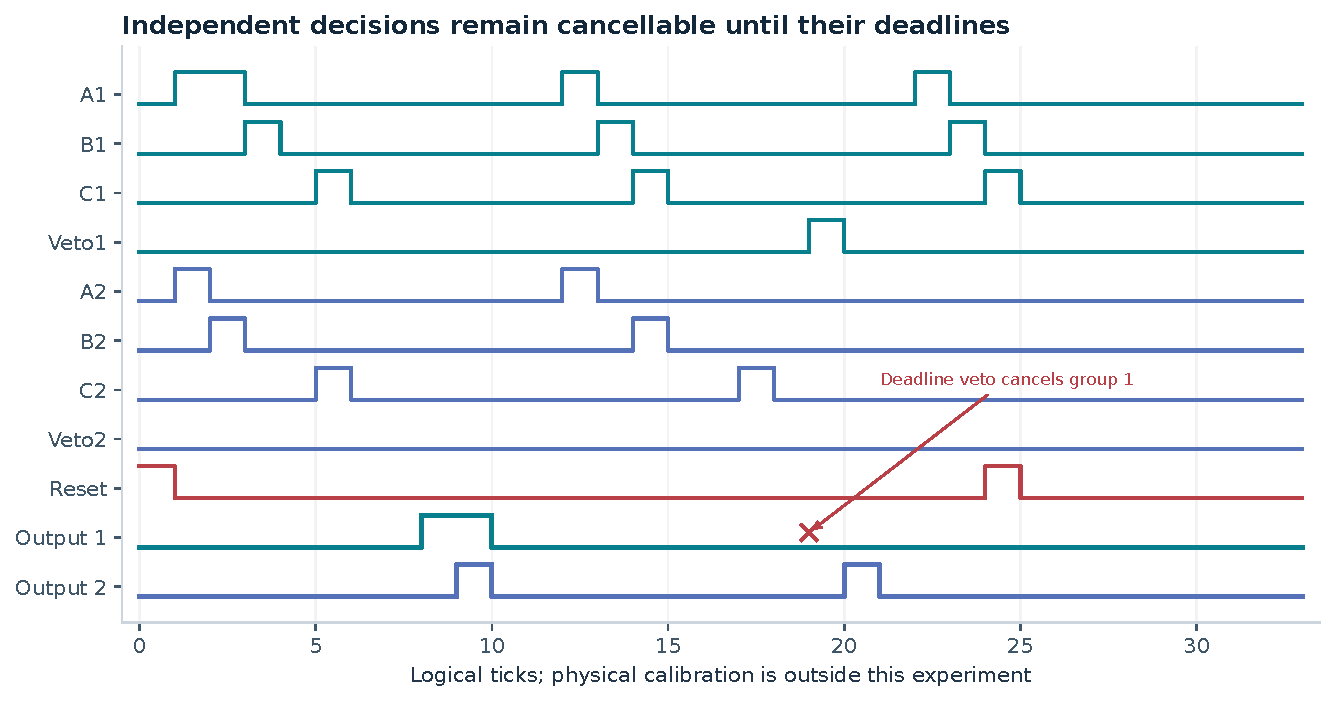
\includegraphics[width=\textwidth]{figures/event_trace.pdf}
\caption{Executed 34-tick demonstration. Group 1 accepts at ticks 8 and 9. Both groups fire at tick 9. A later endpoint veto cancels group 1 at tick 19 while group 2 still accepts at tick 20. Reset at tick 24 clears another pending anchor. Ticks are logical bins, with no physical timing claim.}
\end{figure}

\subsection{The four questions are different}
The campaign asks four questions separately. Does the useful digital capability work? Yes, within the tested contract and bounded proof scope. Can this service sustain a complete enterprise? The selected model says no. Does expert agent operation establish an exclusive advantage? No: the competent conventional control ties functionally and its Python model is faster. Does retained capability help a fresh mission after costs? It provides a working starting point for the network extension, but the identical-library control ties and the US\$4,100 extension is an additional research cost. Those answers can coexist without converting a correct prototype into a fictional breakthrough.

\section{The frontier moved; the commercial bridge still had to be built}
The frontier investigation began with the four requested OpenAI sources, then examined other laboratories and open-source methods. Exact releases were verified before use. The source register distinguishes availability, actual access, limitations and the smallest commercial test for each material advance.

OpenAI's October 6 mathematical collection supplies candidate results and formalization artifacts produced by an internal model; the study did not have that model or reproduce its proof corpus. The October 26 academic-community announcement treats the materials as research inputs and explicitly leaves practical algorithmic consequences for further work. We therefore did not assume a new commercial SAT algorithm from an announcement. The collection was pinned at commit \texttt{7ef5c0cc}; its history also preserves withdrawals and revisions, making version and failure custody part of the investigation.\cite{math,academic,mathrepo}

GPT-6 Astra was released September 3, 2026, and GPT-6.1 Terra October 26. Published standard API prices are respectively US\$10/50 and US\$1/5 per million input/output tokens; Terra cached input is US\$0.05 per million. These prices suggest routing routine intake to a cheaper model and difficult specification work to a stronger one. The session used available Astra agents; Terra was verified in the catalog but not separately benchmarked. No checkpoint identifier or per-task invoice was exposed.\cite{astra,terra,changelog}

\begin{longtable}{L{0.18\textwidth}L{0.22\textwidth}L{0.25\textwidth}L{0.26\textwidth}}
\caption{Frontier register: what changed, what was accessible, and the test needed to make it commercially relevant.}\label{tab:frontier}\\
\toprule Advance / date & Demonstrated or reported capability & Access and limitation in this study & Smallest commercial test \\
\midrule\endfirsthead
\toprule Advance / date & Capability & Access / limit & Commercial test \\
\midrule\endhead
OpenAI math, Oct. 6; collection pinned Oct. 26 & Public manuscripts and some formal proofs at mixed verification stages & Artifacts read; internal generator unavailable; no proof-corpus rerun & Extract one applicable construction and beat a mature finite-instance baseline.\\
Academic communities, Oct. 26 & Public math/CS materials and an external understanding program & Research announcements; physics materials not accessed & Demonstrate a usable algorithm under its exact hypotheses.\\
GPT-6.1 Terra, Oct. 26 & Provider-reported gains in visual reasoning, computer use and cost efficiency & Public release; catalog-listed here, not experimentally compared & Compare cost per accepted intake task, including escalation and repair.\\
GPT-6 Astra, Sept. 3 & Tool-using reasoning, coding and scientific work & Available authoring family; immutable model checkpoint and billing unavailable & Construct the instrument and subject it to independent checks.\\
AlphaEvolve, updated primary report & Evaluator-guided program search across several domains & Public evidence inspected; service not used & A real evaluator must measure the proposed improvement; rivals receive improving AI too.\\
OpenEvolve and formal tools & Open implementations of evaluator-driven search and deterministic verification & Sources examined; standard compiler and Yosys used here & Retain a reproducible executable, not an unsupported model judgment.\\
YoWASP Yosys 0.70, Oct. 13 & Locally executable HDL synthesis, CXXRTL and SAT tooling & Installed version pinned; actual commands and logs preserved & Synthesize and execute both candidates, then prove their bounded equivalence.\\
\bottomrule
\end{longtable}

The broader search included Anthropic's current model documentation, DeepSeek-Prover-V2, OpenEvolve and HiGHS. None was represented as an execution result in this campaign. Their roles were to challenge the notion that exclusive access to one model could sustain an advantage. The full source matrix preserves access distinctions rather than folding every promising announcement into an assumed production system.\cite{alphaevolve,openevolve,deepseek,yosys}

\subsection{The frontier-crossing account}
\textbf{Previously binding constraint:} an uncommon measurement predicate required bespoke specification, implementation and checking, often alongside an existing acquisition system. \textbf{Recent change:} more capable tool-using models and lower-cost routine operation plausibly reduce parts of that construction burden. \textbf{Missing construction:} a bounded event language, a reusable implementation, independent acceptance checks and a support arrangement. \textbf{Newly deliverable outcome in this study:} an executable, checked digital design pack and a composed successor.

This is a candidate \emph{economic} crossing. It is not evidence that temporal logic became technologically possible in 2026. No controlled old-model/new-model trial was performed, so a measured historical cost reduction cannot be assigned to Terra, Astra or AGI in general. The construction succeeded; the complete-cost commercial test determines whether the proposed crossing is enough.

\subsection{The cost-adjusted operating system}
A production design would use inexpensive extraction and administration, selective stronger-model escalation, and deterministic tools for every acceptance-critical step. Once a request falls inside the frozen grammar, compilation and replay need no frontier-model invocation. The model contributes to discovery, specification, code construction and exceptions; the checker supplies reproducible acceptance evidence.

The US\$25 inference allowance per contracted order is an explicit cost estimate for intake and exception handling. It is not charged per clock tick. Shared model/tool development is charged once, and a common defect creates shared repair costs plus customer-specific obligations. Computer operation was used where helpful for file construction, local compilation and browser QA; it does not demonstrate that the native enterprise runtime or a vendor acquisition board was operated.

\section{Discovery before demonstration}
The opening question was: what valuable possibility is now achievable that existing organizations are not equipped to pursue? The second question was: what could we construct that changes the set of possible valuable activities? Five complementary searches produced a diverse shortlist before the selected compiler was implemented.

\begin{longtable}{L{0.18\textwidth}L{0.36\textwidth}L{0.37\textwidth}}
\caption{Five lenses and the evidence they contributed.}\\
\toprule Lens & Opening & Challenge that changed the decision\\
\midrule\endfirsthead
\toprule Lens & Opening & Challenge\\\midrule\endhead
Unmet needs & Precise independent event relationships that an installed filter does not express & The useful outcome must be a specified digital kernel; a whole calibrated instrument cannot be presumed.\\
New capabilities & Current reasoning/coding plus executable verification could shorten bespoke construction & Provider benchmarks do not establish accepted-outcome economics; production routing remains unmeasured.\\
Unexpected combinations & Open acquisition tools, explicit contracts, independent checking and supported reuse & Competent conventional teams and rivals can assemble the same combination.\\
Missing means & A compiler that preserves overlap, endpoints and late veto, with evidence another engineer can replay & Temporal specification-to-FPGA work already exists; the contribution is this bounded delivery construction.\\
Successor possibilities & A verified output becomes an input to a later instrument, extending the accepted grammar & The extension must actually be built, separately frozen, freshly checked and charged.\\
\bottomrule
\end{longtable}

The candidate families included laboratory protocol generation, private cross-owner cohort/aggregate collaboration, shared assay infrastructure, flexible-load capacity arrangements, material/industrial matching, and custom temporal instruments. Protocol generation faced free capable tools and unperformed wet-lab validation. Private collaboration offered consequential benefits but left institutional participation and data access as the central unexecuted dependencies. Shared assays already had substantial community infrastructure. Flexible-load and industrial routes required site evidence and external authority that a local simulator could not supply.

The temporal instrument was selected for a bounded construction campaign because its essential digital capability could be constructed and falsified here, while its commercial weakness could be exposed without pretending that a physical experiment had happened. Constructibility alone did not earn transformational flagship status. The subsequent conventional tie, removal counterfactual and complete-cost failure rejected that stronger claim. The initial selection record is preserved unchanged; a separately dated return-to-search record documents the rejection and renewed comparison.

\subsection{Prior art narrowed the claim}
NIST already provides open-source FPGA acquisition instruments and explicitly supports custom data collection logic. BrightEyes-TTM supplies an open FPGA time-tagging system that has been used in microscopy. These establish practical alternatives, not empty adjacent categories.\cite{nist,brighteyes}

Swabian's Conditional Filter manual, version 2.22.6.0, documents a specific limitation: two independent trigger/filter groups cannot be configured separately in that built-in filter, and cross-triggering can reduce filtering efficiency. Its raw-stream CustomMeasurement and FPGA Link routes nevertheless support custom work. EventWeaver is not claimed to be physically compatible with them; the vendor interface is a separate integration problem.\cite{conditional,rawstream,fpgalink}

Temporal specification-to-FPGA compilation also predates this edition. RTLola work compiles stream-monitoring specifications into synthesizable VHDL; related temporal monitoring systems provide further prior art. Accordingly, this study does not claim invention of temporal monitoring, a universally novel compiler, or an outcome beyond all human foresight. Its non-obviousness claim is limited to an investigated combination and a narrower commercial hypothesis.\cite{rtlola,r2u2}

\subsection{Continuation and active ownership}
The existing AGI Alpha repository and 717 available comments on issue 4850 were inspected. Active studies covered resilient compute placement, conserved production hypotheses, causal capacity and quantitative microscopy image transfer. The last concerns image/coordinate measurement preservation, rather than photon event logic or RTL. No matching temporal-instrument study was found in the inspected coordination record; that search result is not universal absence.

The campaign is additive to pinned main \texttt{12770c22b4a9f90f2013bbfb64242f912ba5071e}. It preserves the exact prior editions and the existing publication owner. A separate source branch and draft review package do not imply canonical Pages publication, merged software qualification or permission to operate deployed contracts.

\section{Constructing the digital instrument}
\subsection{A precise acceptance semantics}
At each logical clock tick $t$, the input is an eight-bit mask. A bit indicates at least one event in that bin; multiplicity within the bin is not represented. A predicate $j$ specifies distinct channels $A_j,B_j,C_j,V_j$, positive inclusive lag bounds $[l_1,u_1]$ and $[l_2,u_2]$, and a deadline $D_j$, with
\begin{equation}
1\le l_1\le u_1,\quad 1\le l_2\le u_2,\quad u_1+u_2\le D_j\le20.
\end{equation}
The output at $t$ is one exactly when an anchor exists at $t-D_j$, an eligible $B$--$C$ path exists, and no veto occurs from anchor through deadline:
\begin{align}
y_j(t)={}& A_j(t-D_j)\ \wedge\ \neg\bigvee_{k=0}^{D_j}V_j(t-D_j+k)\nonumber\\
&\wedge\bigvee_{a=l_1}^{u_1}\ \bigvee_{b=l_2}^{u_2}
\left[B_j(t-D_j+a)\wedge C_j(t-D_j+a+b)\right].\label{eq:contract}
\end{align}
Synchronous reset dominates the mask and clears every pending state. An output after reset needs a complete new history. Positive lag bounds prevent same-tick $A$--$B$ or $B$--$C$ matching, although unrelated channels can coexist in a sample. Multiple paths for one anchor merge to one Boolean result; repeated anchors remain independent. An empty sample advances time. There is no backpressure, implicit timestamp reordering or silent overflow policy: the buyer must supply a lossless clocked-bin interface.

Up to four predicates are supported. They may intentionally share declared channels, but a predicate never reads another group's undeclared channel. The checker rejects malformed names, ranges, channel identifiers, duplicate names, illegal deadlines and unsupported references before emitting a deliverable.

\subsection{The representation that was built}
The compiler uses age-indexed prefix states: surviving anchors, eligible $A$--$B$ prefixes, and completed paths waiting for their final decision. Veto clears all relevant prefixes. The final state stays cancellable through the endpoint. Boolean OR merges alternative paths, preserving the observable answer without counting the same anchor more than once.

Before synthesis, a predicate uses
\begin{equation}
u_1+(u_1-l_1+1)u_2+D_j-l_1-l_2+1
\end{equation}
Boolean state bits. This is a construction formula, not an optimality theorem. Wide windows can make the prefix representation larger than a direct history representation. The independent implementation instead retains event histories and evaluates Equation~\ref{eq:contract} directly. The mathematical oracle scans the event history independently.

The demonstration kernel synthesized to 29 state bits and 73 generic cells: 29 synchronous-reset flip-flops and 44 logic cells, with no latches or unresolved modules. These are generic Yosys statistics, not FPGA lookup-table utilization, physical silicon area, power or clock frequency. Generated C++ was actually compiled and replayed; emitted RTL was actually executed through CXXRTL.

\subsection{What verification establishes}
The checks compare candidate model, conventional model, independent oracle and actual RTL. Bounded SAT miters use explicit initialization/reset assumptions and recorded depths. They establish equivalence over those bounded traces; they do not constitute a universal proof of every possible grammar instance or analog interface. The recurrence provides a useful invariant argument, but the claim remains tied to executed checks and their limits.

The valuable construction is the complete chain from contract to executable behavior to inspectable evidence. An emitted file alone would not satisfy it. Neither would a simulator that assigned successful delivery without executing the essential digital work.

\section{Independent execution and fresh confirmation}
Construction and conventional challenge were assigned to separate workstreams. The conventional implementation received the same event contract, input information and acceptance conditions. It used current AI assistance, direct event-history logic and the same free verification toolchain. It was not deliberately limited to an inferior model or a slower programming language while the candidate received hardware tools.

The main implementation, oracle, comparator and verifier were frozen before an independent entropy seed was selected. Confirmation then generated 24 fresh specifications, each with 32 traces of 256 ticks. The successor received its own source freeze and seed. This separation prevents the successor's new grammar from silently enlarging the predecessor's accepted scope.

\begin{table}[htbp]
\centering\small
\begin{tabular}{L{0.48\textwidth}rr}
\toprule Check & Main instrument & Successor network\\
\midrule
Fresh specifications / networks & 24 & 6\\
Fresh traces passed & 768 / 768 & 48 / 48\\
Logical ticks & 196,608 & 6,144\\
Positive output decisions & 630 & 62\\
Directed cases through actual RTL & 52 & 10\\
Invalid requests rejected & 14 & 9\\
Bounded equivalence checks & 28 & 12\\
Recorded proof depths & 8--22 & 16--34\\
Conventional functional comparison & Tie & Tie\\
Identical-artifact library comparison & Not a main claim & Tie\\
\bottomrule
\end{tabular}
\caption{Executed confirmation. The 491,520 main predicate-tick decisions include multiple predicates per input tick. Directed cases and proof obligations supplement random traces; they do not convert finite coverage into universal physical validation.}
\end{table}

\subsection{A failure that improved the evidence}
The first development run reported apparent one-tick delays in 18 of 32 traces. Both RTL implementations agreed with each other, and bounded equivalence passed. Investigation isolated a CXXRTL driver error: it read combinational outputs immediately after committing state, before a same-clock settling evaluation. The original driver and all failed observations remain preserved. The driver was corrected before freeze, without adding a clock edge, changing the product, or relaxing acceptance. Fresh confirmation used the corrected frozen harness.

This failure matters because agreement between two implementations can conceal a shared observation error. Independent mathematical models and explicit known-answer cases made the discrepancy visible. The final record includes the failure, diagnosis, correction and source hashes; it does not replace the first run with a success-only history.

\subsection{The comparator won an important performance test}
Across the fresh main cases, the EventWeaver Python model took 12.482 seconds, the conventional history model 0.276 seconds, and the offline oracle 0.181 seconds. The candidate Python model was approximately 45 times slower than the conventional model. Paired actual-RTL replay took 0.677 seconds, but that combined replay is not an isolated hardware throughput comparison.

The outcome supports functional correctness and a useful generated design pack. It defeats a broad claim that the prefix model is faster or that this agent-built representation is inherently superior. It also recommends using the simpler conventional model for software-only analysis when it meets the buyer's need. An RTL buyer may still value the complete pack, but that commercial claim must survive the price of the competent alternative.

\subsection{What is necessary for the outcome?}
The proposed transformational kernel is \emph{bounded temporal composition}: independent sequence windows, an inclusive veto interval that remains open until the decision deadline, and a decided event that can become a later instrument's input. These functions are exercised by the offered design pack. Their necessity for a selected contract must be distinguished from the necessity of our implementation, scientific novelty, or a newly viable business.

We therefore declared a separate, postconfirmation ablation protocol. Six explicit traces, the exact operator removals, the expected outputs, the comparison methods and the stopping rule were frozen at 14:19:23 UTC on 28 October 2026, before the ablation run. The retained main compiler, successor, independent conventional implementations, oracle and verifiers were checked against their recorded source hashes before and after execution; all remained unchanged. This extension does not enlarge the original fresh-confirmation sample.

The first mutation accepts an anchor irreversibly at its earliest valid C event, without waiting for future vetoes. The second pools all declared A channels, all B channels, all C channels and all veto channels across groups while retaining each predicate's own lag bounds. The third disconnects every virtual event by setting it to zero, preserving raw inputs and stage logic. Each mutation was executed both as a Python model and as generated RTL evaluated through Yosys CXXRTL. The full implementation was also compared with the independent oracle and conventional RTL on exactly the same traces.

\begin{table}[htbp]
\centering\small
\begin{tabular}{L{0.35\textwidth}L{0.25\textwidth}L{0.25\textwidth}}
\toprule Predeclared fixture & Full contract & Operator removed\\
\midrule
Late veto at tick 7 & No output & $0@2$ (false acceptance)\\
Same sequence, no veto & $0@7$ & $0@2$ (wrong time)\\
Events drawn from different groups & No output & $0@7,\;1@8$\\
Valid independent groups & $0@7,\;1@8$ & $0@7,\;1@8$\\
Virtual event activates second predicate & $0@8,\;1@14$ & $0@8$ only\\
Raw-stage control & $0@8$ & $0@8$\\
\bottomrule
\end{tabular}
\caption{Kernel counterfactuals. The notation $j@t$ means output bit $j$ at zero-based logical tick $t$. All six fixtures and 88 ticks matched their predeclared full and mutated outputs in executable models and actual RTL. The no-veto control preserves the existence of a match but reveals the early-accept mutation's changed decision time. No unexpected error occurred.}
\end{table}

\textbf{Removing our compiler did not remove the outcome.} Substituting the independently implemented conventional history-formula RTL, including the conventional successor network, preserved every result in all six fixtures. This counterfactual defeats a claim that EventWeaver itself was necessary for these outcomes. Temporal composition is a functional requirement of the selected contracts; EventWeaver is one implemented means of satisfying it. Existing conventional software and custom digital logic remain strong alternatives.

The result is therefore a tested construction with a necessary \emph{semantic} kernel, not an earned claim of exclusive transformational capability. The fixtures were deliberately chosen to expose the specified removals. They are not a blinded causal experiment on agent skill, a random estimate of field failure, or evidence that current frontier intelligence uniquely made the commercial opportunity feasible. Nor does an ablation establish customer willingness to pay. Full traces, source integrity records, generated mutant RTL and discrepancies are retained in \texttt{protocol/kernel\_ablation\_v1.json}, \texttt{protocol/kernel\_ablation\_freeze.json}, and \texttt{results/kernel\_ablation.json}.


\subsection{Independence and its limits}
The verifier and conventional code were separately authored rather than copied from the candidate. The ledger auditor imports neither the business simulator nor its accounting helpers. Nevertheless, these are separate AI-assisted workstreams in one campaign, with shared model-family risks. They are not a blinded human laboratory review, an independent customer acceptance, or a formal proof of every implementation layer. No human-specialist advantage is inferred from their agreement.

\section{The complete commercial offering}
\subsection{Scope that can be sold honestly}
The offering is a supported functional design pack for a bounded event contract. It contains validated specifications, generated source, reference behavior, independent acceptance evidence and limited support. The published compiler can be reused freely; the selected US\$1,200 fee is for service and accountable delivery, not an invented exclusive license over public source.

Qualification requires an existing digitized event interface, a request inside the grammar, a named acceptance authority, an actual need beyond installed functions, and a budget that survives comparison with internal/current-AI work. Requests for analog timing, vendor-link integration, safety-critical certification, unlimited predicates or unsupported timestamp semantics are refused or require a separate study. The commercial simulator never makes those missing capabilities succeed behind the scenes.

The modeled contract uses a 40\% refundable deposit, restricted until acceptance. The balance is due 60 days after acceptance, with modeled procurement and payment delays. A 45-day warranty permits repair, invoice credit and cash refunds. A 42-day delivery deadline applies to the contract, including pool formation and correction. Source and evidence are supplied under the declared rights; later revalidation is a separate US\$450 renewal service, chosen only when buyer utility and seller contribution justify it.

These are research contract terms rather than advice about enforceability in a particular jurisdiction. In particular, a buyer who has received source may strategically withhold the balance if enforcement, reputation and continuing-support incentives are absent. That payment-stage deviation is tested explicitly.

\subsection{Acquisition through exit}
The acquisition window lasts 180 days. The base assumptions begin with 180 scoped prospects, an 18\% inquiry probability, and 62\% qualification among inquiries. Marketing, failed qualification, quotations, negotiations and procurement refusals all consume resources. The proposal does not assume an unlimited queue of willing buyers.

The event simulation then executes contracting, restricted deposit custody, capacity/funding admission, implementation, initial acceptance or refusal, bounded correction, final acceptance or refund, support, warranty, collection or default, renewal quotation, renewal acceptance or refusal, and exit. Administration continues during runoff. The allowed horizon is 730 days; the latest base obligation occurs by day 450. No new intake continues indefinitely to conceal a losing first campaign.

Renewals have a narrower modeled lifecycle: after the utility and procurement gates, the simulator assumes accepted revalidation and full collection. It does not add a second technical-failure, correction, warranty or default cycle. This optimistic renewal assumption does not rescue the losing policy; it limits any claim that all repeat-delivery risks were tested.

One illustrative history was selected \emph{after} confirmation to show lifecycle behavior; it is not representative evidence chosen to optimize the result. In seed 700587, buyer B0034 negotiated US\$1,127.83, paid a US\$451.13 restricted deposit on day 18, initially refused the pack on day 20, accepted a correction under the unchanged contract on day 21, received support, and paid the US\$676.70 balance on day 129. The warranty closed on day 66 and the buyer did not renew. The same history includes defaults and full warranty refunds.

Buyer B0018 illustrates why acceptance and collection must remain distinct. A full warranty refund credited the remaining US\$688.96 receivable and returned the US\$459.31 already released deposit. Its later collection event simply closed a zero invoice balance; it was not another receipt. Buyer B0008 defaulted on US\$670.07, which remained a bad-debt cost. Dollar ledgers, rather than lifecycle event counts, determine revenue and cash.

\subsection{Buyer objectives, information and alternatives}
For buyer $i$ and alternative $a$, the model evaluates
\begin{equation}
U_i(a)=q_a V_i-p_a-w_i h_{ia}-\tau_i d_{ia}-T_{ia}-R_{ia},\label{eq:utility}
\end{equation}
where $V_i$ is the assumed value of a successful digital outcome, $q_a$ a belief about success, $p_a$ the price, $h_{ia}$ internal effort, $d_{ia}$ delay, $T_{ia}$ trust/onboarding burden, and $R_{ia}$ reuse-rights or setup burden. Buyers choose among the offering, a competitor, internal current-AI-assisted engineering, free tooling, waiting, and doing nothing. The last alternative has utility zero.

Gross value has a modeled median of US\$6,500, but this does not set the selling price. The strongest feasible outside utility limits the buyer's reservation price. Internal work uses six to sixteen design hours plus four to eight review hours; competitor quotes range from US\$1,500 to US\$3,300 before response factors. Both are explicit estimates for this small digital scope, not prices for a complete optical instrument. Supplier labor is anchored to public wage data and then increased to an assumed US\$135 per hour for specialist/business cost.\cite{bls,ecec}

The buyer privately knows its modeled value and outside cost and submits a bounded counter-bid. The seller observes that bid and its own expected incremental obligation, not the buyer's hidden reservation price. It refuses a bid below the cost gate or a contract beyond available capital commitments. This is a specified bargaining heuristic, not an incentive-compatibility theorem. Logged utilities, bids, prices and decisions allow an independent auditor to reconstruct the choices.

Modeled participation and a positive utility value are not independent willingness-to-pay evidence. They say what follows from the stated assumptions. The commercial gate remains actual buyer evidence.

\section{Inventing the arrangement, then testing its incentives}
\subsection{Three arrangements and a bounded price search}
Development compared three arrangements at posted fees of US\$1,200, 1,800, 2,400, 3,000 and 3,600. Each policy used 96 development seeds before the selection was frozen.

\textbf{Bespoke service} supplies more seller construction effort and less buyer setup. \textbf{Three-order pooling} shares a validation batch and requires nonexclusive core rights, explicit coordination, and a 28-day formation window. Unformed groups receive deposit refunds. \textbf{Supported library} uses retained source with fewer seller construction hours and more buyer-side setup. The buyer's extra work remains in Equation~\ref{eq:utility}; it is not silently moved out of the comparison.

Pooling creates a potential gain by avoiding repeated core validation. It also creates waiting, coordination, withdrawal and correlated-defect costs. Each participant must prefer the pooled outcome to its own best alternative. A buyer who will not share reuse rights pays the opportunity cost or chooses another route. Generic-core benefits can be copied by competitors, so the same pooled arrangement is available in the conventional strategic comparison.

All 15 development policies lost full-project money. The least-loss policy was the supported library at US\$1,200. It was frozen for research confirmation, not approved for launch. The option \emph{do not launch} has zero incremental project profit and dominates those launch policies under their development assumptions.

\begin{figure}[htbp]
\centering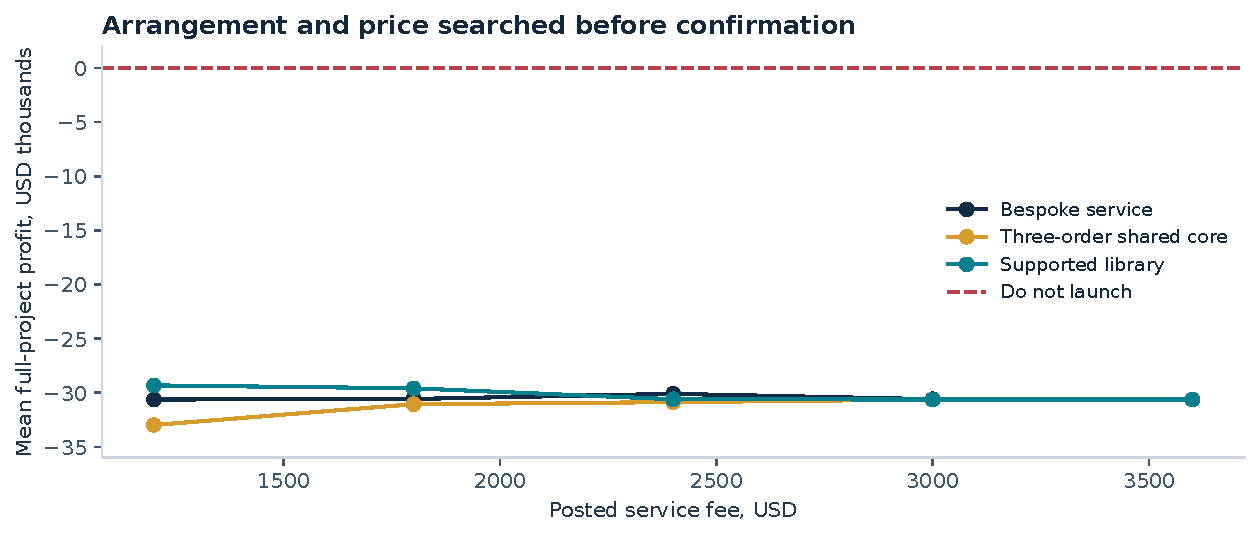
\includegraphics[width=\textwidth]{figures/development_policies.pdf}
\caption{Bounded price and arrangement search before confirmation. The horizontal zero-profit line is the no-launch outside action. A price that loses fewer dollars is not a commercially viable optimum.}
\end{figure}

\subsection{Competition and strategic behavior}
The lifecycle model includes a competitor price reduction, identical public-library access, and a conditional AI-improvement scenario for both seller and rivals. It does not assume that frontier progress belongs exclusively to this enterprise. Supplier quotes above a fixed US\$180-per-hour reservation are refused; capacity and rate shocks can therefore reduce activity rather than magically increase prices buyers will pay.

A separate finite price game makes the strategic issue explicit. Four thousand synthetic buyer types define a distribution of outside options; two firms post prices on a US\$900--3,000 grid and may decline entry. Both receive the same cost reduction when shared-core delivery is available. The entrant bears US\$23,000 of initial research construction; the incumbent's incremental fixed entry cost is zero. These are stylized assumptions, not an estimated market equilibrium.

Conditional on both firms remaining active, the individual-delivery game has two pure equilibria, at entrant/rival prices US\$900/1,200 and US\$1,200/1,500. Entrant profits remain negative. Allowing entry refusal yields no entry by the new firm and a US\$2,100 incumbent price on this finite grid. A shared-core cost reduction available to both does not change the no-entry conclusion. A bounded-rational logit response check also concentrates on exit. Independent reconstruction verified all 324 payoff cells and the reported best-response sets.

The game cannot identify unknown demand, customer value or enforcement costs. Its purpose is to test whether a claimed arrangement gain survives strategic access by rivals. It provides no reason to turn an unsupported demand assumption into a fact.

\subsection{The collection subgame and loss-leading claims}
After final source delivery, an opportunistic buyer may save the unpaid balance by defaulting. Compliance requires the expected enforcement, reputation or lost-support cost to exceed that saving. With a hypothetical US\$1,140 fee and a 40\% deposit, US\$684 remains exposed. The simulator's normal collection behavior is an assumption; the no-recourse stress defaults every postdelivery balance. Inspection-compatible escrow or payment before final-source handoff might improve incentives, but would change the contract and buyer participation and therefore requires a new frozen study.

The campaign also rejects an unsupported loss-leader argument. There is no observed downstream order book that can justify today's loss. Successor value is not booked as revenue, an asset uplift, or a second source of funding. The US\$4,100 research extension is charged once. A milestone may rationally lose money when a bounded, independently evidenced downstream benefit exceeds that loss; no such evidence was established here.

\section{Closing costs, cash and uncertainty}
\subsection{What the complete bill contains}
The full campaign includes discovery, failed attempts, core construction, independent verification, tools/data/compute, estimated inference, contract design, artifact extraction, the successor research option, acquisition, qualification, quotation, procurement, delivery, correction, support, common repair, warranty, bad debt, renewals, administration and financing. Shared construction is allocated once. The modeled US\$23,000 startup bill includes US\$4,100 for succession; acquisition-window fixed overhead adds US\$2,700. Later runoff administration is charged separately.

The selected policy uses three seller delivery hours per order, plus explicit qualification, support, repair and renewal work. It reserves eight additional delivery-capacity hours per order for obligations. That reserve is a conservative aggregate scheduling proxy; it is not a verified weekly support service level. Sales capacity is separately limited. Fixed research labor is charged in startup costs and is not misrepresented as measured human time.

\begin{table}[htbp]
\centering\small
\begin{tabular}{L{0.55\textwidth}r}
\toprule Fresh base result, 1,024 histories & Mean\\
\midrule
Accepted initial design packs & 7.94\\
Net recognized revenue & US\$9,024\\
Net customer cash after refunds and defaults & US\$8,836\\
Complete project expense & US\$38,653\\
Operating contribution before fixed costs and financing & US\$\(-3,928\)\\
Full-project profit & US\$\(-29,628\)\\
Return on total cost, ratio of means & \(-76.7\%\)\\
Mean unrestricted capital required & US\$32,111\\
95th percentile unrestricted capital required & US\$36,496\\
Mean variable human service hours & 72.81\\
Variable service hours per accepted outcome & 9.17\\
Modeled interventions per accepted outcome & 1.19\\
\bottomrule
\end{tabular}
\caption{Recognition, collections, operating contribution, full-project profit and capital are distinct. Human hours and interventions are explicit commercial assumptions; technical trace counts and tool runtimes are executed measurements.}
\end{table}

The average modeled buyer benefit conditional on participating histories is approximately US\$359 before realized outcomes, relative to the best modeled outside alternative. That is an output of assumed private values and delays, not measured customer savings. The selected service can benefit some modeled buyers while the enterprise loses after acquisition and fixed costs.

\begin{figure}[htbp]
\centering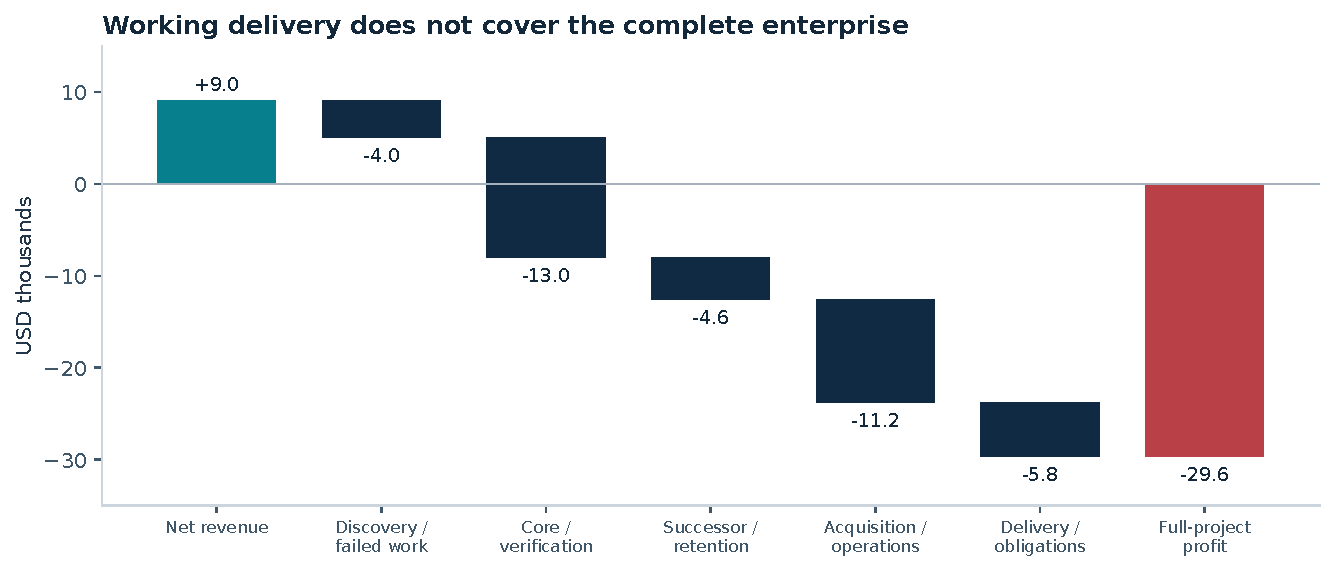
\includegraphics[width=\textwidth]{figures/economics_waterfall.pdf}
\caption{Complete-cost bridge for the frozen base policy. Operating losses remain even before the fixed research bill. Artifact retention and successor development are visible costs.}
\end{figure}

\subsection{Accounting and financing}
The journal uses integer cents and double-entry postings. A deposit debits restricted cash and credits a liability; it is not revenue or available working capital. Acceptance recognizes a receivable and revenue, applies the deposit against that receivable, and releases only the corresponding restricted cash. Collection exchanges receivables for cash without recognizing revenue again. Warranty first credits unpaid receivables and then refunds already collected cash. Defaults are bad debt, not invisible missing receipts.

The policy starts with US\$45,000 equity and a US\$15,000 credit ceiling at a 12\% annual rate. Contract admission uses recorded commitments and excludes refundable deposits. The reported required capital is the peak unrestricted deficit before financing, not hindsight used to approve contracts. The model permits an explicit emergency-equity requirement to register a funding failure; it does not turn such a requirement into successful free capital.

In base confirmation, no emergency injection or debt draw was required, and all modeled obligations settled. The broader stress campaign contains seven terminal insolvencies: one no-recourse history retains US\$2,524.62 of debt, and six high-demand histories retain US\$6,285.11 in aggregate across separate histories. These liabilities are not forgiven. Customer deposits, receivables and refunds close, but universal financing closure is not claimed. Unpaid debt is measured at each terminal date; later interest, creditor recovery and insolvency resolution are not simulated.

\subsection{Risk is conditional on the model}
Every base history lost money. The base 5th--95th percentile profit interval is US\$\(-34,181\) to US\$\(-26,599\); the mean of the worst five percent is US\$\(-36,449\). The Monte Carlo standard error of mean profit is about US\$76. The conditional 95\% Wilson interval for the sampled loss probability is 99.626\%--100\%.

That narrow interval quantifies sampling precision \emph{inside this model}. It does not measure real-world certainty about demand, buyer value, scope fit, support burden or competitor behavior. The cash-shortfall estimate is zero in the base sample, with a sampling upper bound of about 0.374\%, under the stated capital policy. It is not a promise that an actual enterprise needs no contingency capital.

\begin{figure}[htbp]
\centering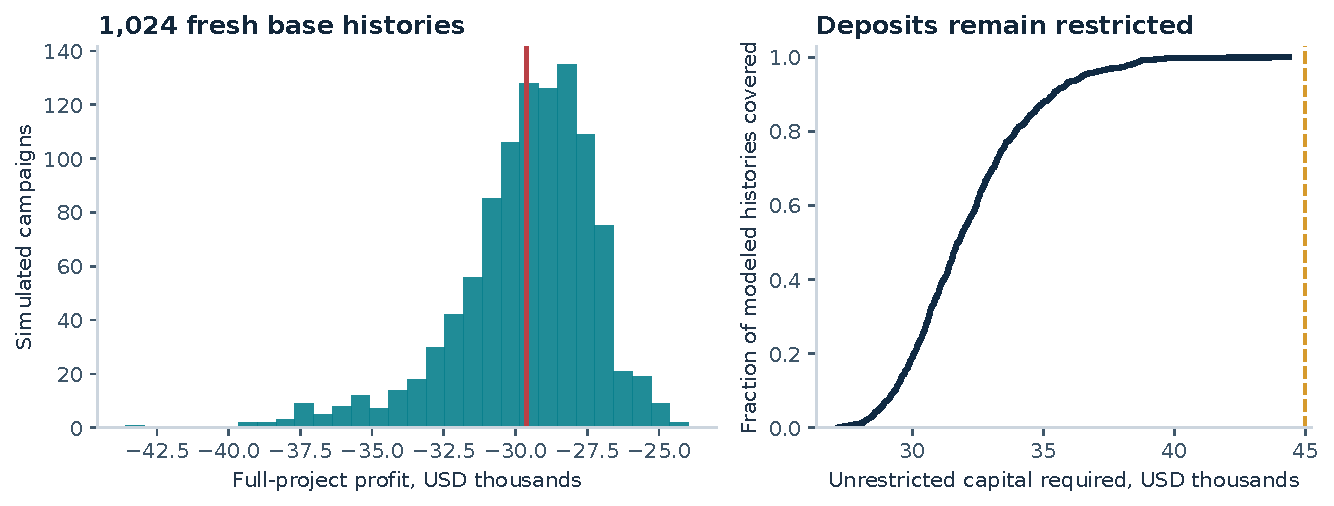
\includegraphics[width=\textwidth]{figures/uncertainty_cash.pdf}
\caption{Profit dispersion and capital coverage within the frozen base model. The dashed capital line marks US\$45,000 equity; refundable deposits are excluded. Model uncertainty is broader than these Monte Carlo distributions.}
\end{figure}

\begin{table}[htbp]
\centering\small
\begin{tabular}{L{0.57\textwidth}rr}
\toprule Conditional scenario, 1,024 histories each & Mean profit (US\$) & Accepted packs\\
\midrule
Base & \(-29,628\) & 7.94\\
Competitor price response & \(-30,410\) & 3.72\\
Weak demand & \(-28,305\) & 3.91\\
Supplier cost/capacity shock & \(-32,636\) & 0.79\\
Slow payment and more defaults & \(-30,195\) & 7.94\\
Correlated downturn & \(-30,397\) & 1.06\\
Identical free library & \(-30,767\) & 0.00\\
Conditional AI improvement for all firms & \(-30,721\) & 1.02\\
No collection recourse & \(-34,629\) & 7.94\\
2.5 times demand, fixed capacity & \(-33,810\) & 11.99\\
\bottomrule
\end{tabular}
\caption{All ten scenarios lose in every sampled history. No probabilities are assigned across scenarios, so the rows must not be averaged into an unconditional forecast.}
\end{table}

\begin{figure}[htbp]
\centering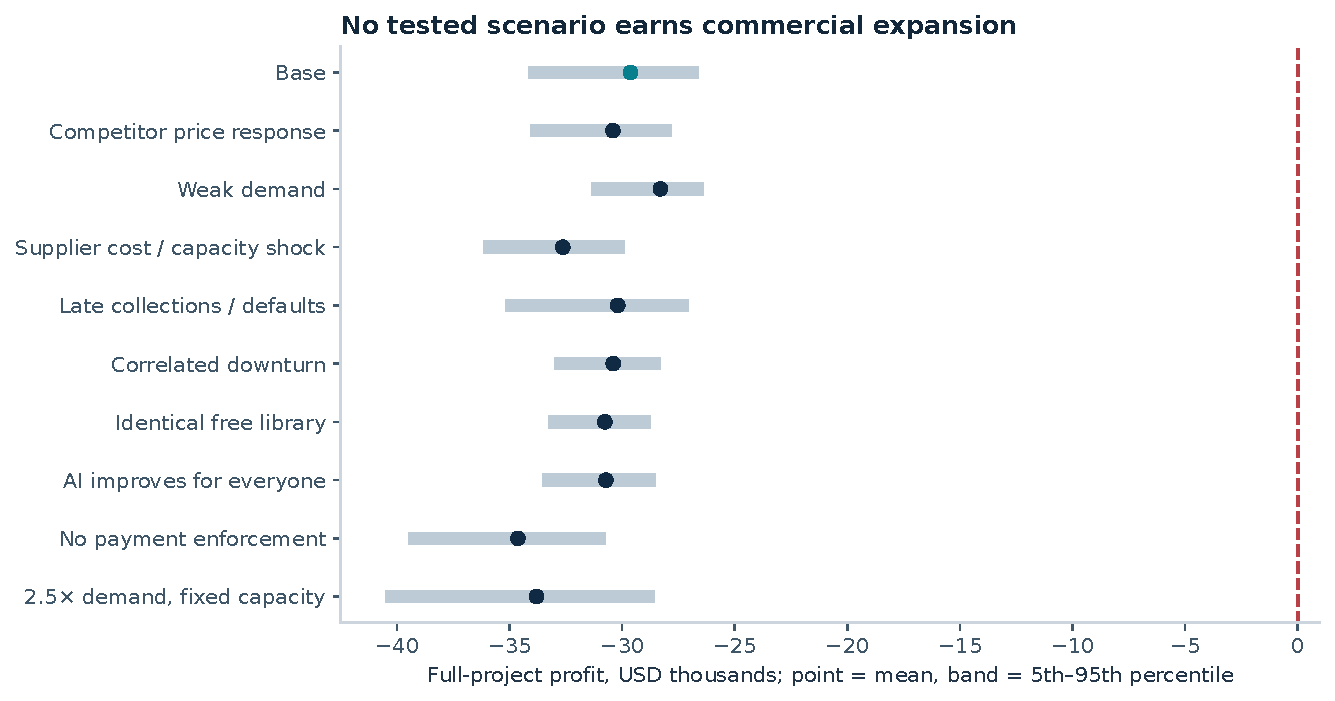
\includegraphics[width=\textwidth]{figures/scenario_results.pdf}
\caption{Mean and 5th--95th percentile profit by scenario. Higher demand creates more acquisition and obligation costs; cheaper AI also strengthens outside options. Neither is assumed to rescue the offering.}
\end{figure}

\subsection{Break-even demand, price, acceptance and cost}
At the observed simulated mix, net revenue including renewals is about US\$1,136 per accepted initial pack, and direct cost including failed work is about US\$735, leaving roughly US\$401 before other campaign costs. Holding that mix fixed gives an optimistic arithmetic break-even requirement of \textbf{82 accepted packs}. The 180-day reserved-capacity ceiling is about 42 orders before failures, sales limits and renewal work. Customer acquisition and support costs would also change with volume; 82 is a diagnostic lower hurdle, not a growth projection.

Holding the approximately eight accepted orders fixed, the mean negotiated price would need to rise from about US\$1,153 to roughly \textbf{US\$4,883} to cover the loss. The development demand response already collapses at much lower posted fees. A fixed discount from a complete instrument's price would therefore be an invalid pricing argument.

Acceptance alone cannot close the gap. Even accepting every currently contracted order at the posted fee, before any variable cost, does not cover the US\$25,700 fixed campaign bill. Eliminating all direct delivery cost still leaves other project costs above net revenue. Eliminating inference charges alone saves only a small fraction of the loss. The constraint is the supported service's complete economic arrangement, not merely a residual model error rate.

\section{Autonomy, capacity and the billion-plus hurdle}
The implemented compiler performs ordinary in-grammar construction without another model call. Validation, replay and acceptance checks are executable. The demonstration and fresh cases were processed automatically once their contracts existed. This is meaningful technical automation, but it does not establish an unattended enterprise: prospect qualification, semantic agreement, buyer authority, exceptions and support remain commercially consequential work.

The model assigns approximately 1.19 human intervention events and 9.17 variable service hours per accepted initial outcome. These are separate quantities: a review intervention can consume hours, and unsuccessful prospects consume effort without creating an accepted outcome. Fixed discovery and research labor is already included in the monetary startup bill. The campaign did not measure a real customer's required human attention, nor infer it from zero human clicks in a synthetic replay.

\subsection{Where the queues bind}
The policy allows eighteen delivery-capacity hours per week and six separately reserved sales/qualification hours. Supported-library orders require three direct construction hours plus an eight-hour aggregate reserve for support, warranty and later obligations. Formation waiting, funding refusal, correction and a contract-level deadline remain visible. The reserve is deliberately conservative, but it does not model a detailed multi-person calendar or prove response-time guarantees during a common incident.

At this reservation rate, one delivery resource has a theoretical ceiling of about 42 orders over 180 days, or 85 per year, before failure, acquisition and renewal constraints. High demand increases accepted orders only from about 7.94 to 11.99 in the tested scenario and increases the expected loss. More agents do not remove buyer acquisition, specialist review, contractual trust or capital obligations. Scaling requires an evidenced change in those constraints.

\subsection{A large industry is not a qualified market}
Primary industry sources provide useful context but not a measured addressable market for this grammar. SPIE's February 2026 issuer release reports roughly 1,600 Photonics West exhibitors and US\$381 billion in 2024 core-component revenue. Photonics21's 2024 report identifies a much broader US\$16 billion instrumentation/optical-measurement category in 2022. Those organizations, definitions and revenue categories cannot be added, and neither establishes eligible EventWeaver customers.\cite{spie,photonics21}

An illustrative funnel of 1,600 directory firms, 10\% eligible, 25\% adopting and two orders per year produces 80 orders and US\$96,000 gross annual revenue. Every funnel fraction is an assumption. At the frozen fee, US\$1 billion in annual revenue would require 833,334 accepted packs. The current narrow offering does not support that volume or its acquisition and service requirements.

The explicit long-horizon ambition is instead \textbf{US\$1 billion of annual net incremental productive value in 2031, measured in constant 2026 dollars relative to the strongest feasible alternative}. A possible arithmetic decomposition is
\begin{equation}
10{,}000\ \text{deployed instruments}\times
\mathrm{US}\$100{,}000\ \text{net annual benefit per instrument}
=\mathrm{US}\$1\ \text{billion/year}.
\end{equation}
Neither adoption nor attributable benefit has been evidenced. Revenue, profit, productive value and valuation are distinct; no valuation is derived from this identity. A route through OEM distribution or a new instrument family would need demonstrated integration, reachable deployments, measured productivity and benefit-sharing terms. The present campaign does not earn a defensible billion-plus thesis.

\section{The successor received a new starting point}
\subsection{A fresh mission that changes the grammar}
The original compiler accepts raw event channel numbers. Its successor adds named virtual references, such as \texttt{stage:heralded\_probe}, allowing an accepted instrument decision to serve as a later instrument's event. The new mission is a heralded detection followed by a conditionally activated calibration-trigger event sequence on other channels. Only Boolean event logic is implemented; no physical calibration is performed. This is a compositional extension, not merely a different lag value or more copies of a supported predicate.

The network must be acyclic, names must resolve, and each consumer observes the previous tick's producer output. All stages read that previous-output snapshot and then update simultaneously. Reset clears the entire network. The original compiler's rejection of virtual references is explicitly tested, establishing that the new wrapper supplies a capability outside its accepted input grammar.

\begin{figure}[htbp]
\centering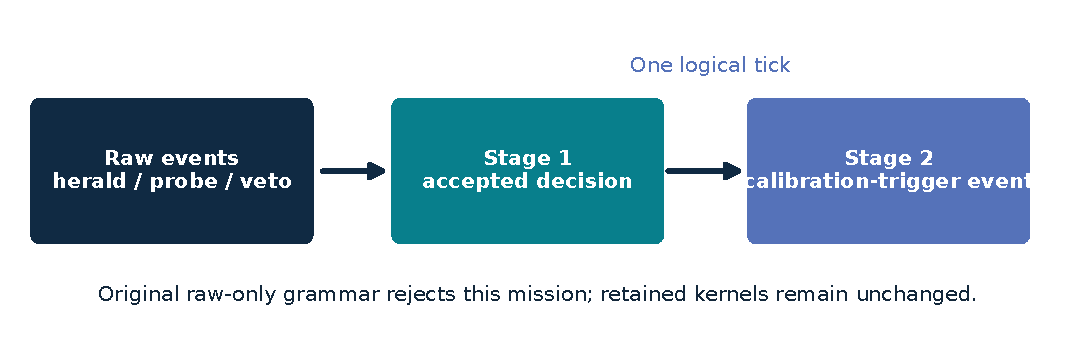
\includegraphics[width=\textwidth]{figures/successor_network.pdf}
\caption{The successor composes unchanged, source-bound kernels through a new acyclic virtual-event interface. One logical tick of interface delay is part of acceptance, not an implementation detail the buyer must guess.}
\end{figure}

The first stage in the demonstration accepts at tick 8; its virtual event reaches the consumer at tick 9; the conditioned stage accepts at tick 14. A later deadline veto cancels a second conditioned decision. Direct RTL wiring between synchronous kernels supplies the previous edge's output; adding another register would incorrectly create a second interface tick.

The demonstration network synthesized to 25 state bits and 65 functional generic cells, plus two Yosys metadata cells. Fresh confirmation used six previously unseen networks and 48 traces, with 10 directed actual-RTL cases covering virtual references in $A$, $B$, $C$ and veto roles, reversed listing order, reset, endpoint veto and a three-stage chain. Twelve bounded equivalence checks passed at depths 16--34.

\subsection{What was inherited, what was rebuilt, what it cost}
The retained asset is the exact predecessor compiler, identified by SHA-256. The wrapper checks that identity. New work includes network grammar validation, virtual-event mapping, graph checks, composition semantics and independent network verification. An ordinary library containing byte-identical compiler and wrapper files was executed in an isolated subprocess and tied. A conventional network wrapping independently authored history kernels also tied functionally.

This result demonstrates productive reuse and a new supported mission. It does not show learned weights, an independently superior specialist or a benefit unavailable from ordinary software reuse. The evidence supports selecting a useful retained artifact, not equating storage with learning.

The extension is charged at US\$3,500 for grammar/integration, validation, fixtures, inference/tools and a failure allowance, plus US\$600 for extraction, validation, integration and first-year storage/upkeep. The total US\$4,100 is included once in the campaign startup account. The conventional identical-library route bears the same retention costs. No commercial surplus funded this extension; it was a separately costed research option within the campaign.

\subsection{The two connected flywheels}
The transformational path has executed links: frontier investigation led to a construction; the construction produced a verified digital capability; that retained capability supported a new compositional instrument. The commercial path reaches an offering and modeled delivery, but stalls before complete-cost surplus. Its missing link cannot be supplied by calling the successor a valuable asset or assuming future growth.

\begin{figure}[htbp]
\centering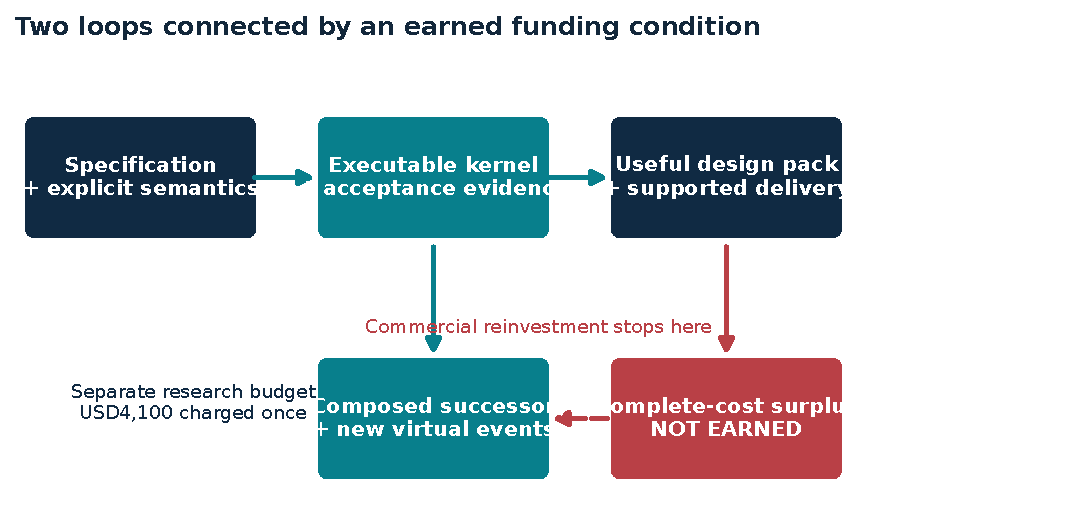
\includegraphics[width=\textwidth]{figures/two_flywheels.pdf}
\caption{The experiment constructs the technical succession link and exposes the unclosed commercial link. A separate research budget is not self-financed compounding.}
\end{figure}

Future surplus would first need to fund buyer-specific interface qualification, timing/throughput evidence, reusable adapters and continued validation. Those means might unlock an integrated measurement offering that this functional kernel cannot yet deliver. The opportunity would support further useful work only if buyers value the integrated outcome above their alternatives and its complete obligations. Neither reinvestment success nor exponential growth is assumed.

\section{Decision: stop this launch and reopen the search}
\textbf{Stop standalone expansion of the frozen US\$1,200 supported-library offering.} The useful construction passes its bounded technical tests, but all tested commercial policies fail to cover full costs and the selected policy loses even before fixed campaign costs. Conventional parity, the negative Python timing result, free-library access and unmeasured demand all constrain the advantage claim.

This is not a proof that every instrumentation enterprise is uneconomic. It is a decision about the selected scope, price, arrangement, acquisition assumptions and obligations. A larger integration problem might justify a different contract and price, but its value cannot be assigned to the small kernel already tested.

\subsection{The failed candidate did not retain the flagship}
After the complete-cost rejection, the campaign returned to the wider possibility search. This was a new, bounded desk investigation recorded on October 28, with priority given to the preceding thirty days and seven days. It did not alter the original selection record, frozen commercial policy or confirmation histories. The stronger question was: what productive capability could change the available actions, and would removing that capability destroy the first valuable outcome?

This \textbf{OUT-TRANSFORM} lens starts with a desired possibility, identifies its binding constraint, invents the means that could remove it, and then asks for a first commercial outcome that actually depends on those means. It does not promote an advisory report or acceptance wrapper when the essential physical or institutional construction is missing. Three serious hypotheses were compared independently of the completed compiler's sunk cost.

\begin{longtable}{L{.21\textwidth}L{.34\textwidth}L{.36\textwidth}}
\caption{Reopened search: consequential possibilities, essential delivery and rejection. The candidates are hypotheses; no second physical or institutional experiment is claimed.}\\
\toprule Possibility & First outcome that requires the construction & Binding gap and campaign decision\\
\midrule\endfirsthead
\toprule Possibility & Essential first outcome & Gap and decision\\\midrule\endhead
Counterfactual experience foundry & A robot recovery controller that succeeds on withheld physical interactions, built from a calibrated generator of scarce training experiences & No robot, physical calibration, model execution, transfer result or paying task. Strongest next investigation, but rejected as this edition's flagship.\\
Local-feedstock material commons & A physically manufactured and tested recipe makes a previously unsuitable local feedstock usable within a declared performance envelope & No samples, assays, accepting producer or complete physical delivery cost. A recipe report would omit the kernel. Reject.\\
Private cross-owner experimental instrument & An authorized joint experiment yields an accepted conclusion that no owner can obtain alone under the same disclosure constraints & No authorized consortium, harmonized measurements or required operation beyond strong free stacks. Synthetic parties would erase the key barrier. Reject.\\
\bottomrule
\end{longtable}

\subsection{The strongest conditional opening: produce informative experience}
The blue-sky possibility is that robots can acquire useful recovery skills from experiences too rare, expensive or destructive to stage repeatedly. The productive object is trustworthy, action-conditioned experience with transferable outcomes. A pile of plausible videos is insufficient. The proposed means is a task-specific world-model/physics hybrid that identifies uncertain physical parameters, generates discriminating recovery interactions, and trains a bounded controller with an explicit validity envelope.

Fresh primary evidence makes this worth investigating. NVIDIA's October 21 Cosmos announcement adds public training tools, simulation checkpoints and Data Factory blueprints. Its repository already includes generation and validation workflows, so those are also incumbent alternatives. Google announced Genie 4 on October 27 as a trusted-tester research preview, with acknowledged physical, spatial and long-session consistency limitations. Gemini Robotics Embodied Reasoning 2 entered public preview the same day, providing high-level reasoning and orchestration that still depends on low-level control interfaces and physical deployment. None of these models was executed in the reopened search.\cite{cosmos,cosmosfactory,genie4,roboticser2}

The first offer would serve one integrator-owned fixture: deliver a recovery controller and calibrated experience generator that achieve an agreed jam/slip recovery on withheld physical instances under fixed time and intervention limits. The buyer is the integrator accountable for throughput. Its strongest alternatives include open Cosmos tooling, competent conventional simulation/domain randomization, demonstration learning and a current-AI-assisted robotics engineer.

The removal test is decisive: hold real data, compute, engineer effort and acceptance fixed, then remove the calibrated counterfactual-generation and parameter-identification loop. An attributed recovery gain should disappear. Replacing a branded tool with a competent substitute must also be tested. If conventional simulation ties at equal or lower complete cost, exclusive kernel advantage fails; a useful integration business would still need independent commercial evidence.

\textbf{No product or paid pilot is claimed.} The campaign had no fixture, physical trace set, calibration or measured buyer benefit. A local analytic or MuJoCo surrogate could test code plumbing, but it would not establish the physical-transfer outcome sold by this offer. Reopening requires actual usable fixture/data access, a named accepting operator, matched baseline and a capped complete-cost experiment. This record does not invent a price, market size or rare-success payoff to manufacture a positive business case.

\subsection{Why the other openings were also rejected}
The local-materials hypothesis would change which heterogeneous feedstocks can be used, through adaptive characterization, recipe generation and batch qualification. The October 20 Saint-Gobain/Microsoft account reports accelerated knowledge construction and hypotheses worth testing; it does not establish our proposed recipe, qualification result or economics. A fair next experiment would make held-out batches from independent feedstock lots and compare conventional experimental design on the same assays, charging failures, disposal and retesting. No such physical construction occurred here.\cite{saintgobain}

The cross-owner hypothesis would change the available scientific action from isolated analysis to an authorized joint experiment. Its missing means includes disclosure control, compatible measurements, governance and participant incentives. DataSHIELD already supplies mature federated analysis with disclosure checks; SecretFlow supplies established secure-aggregation methods. Microsoft's September 29 Quine announcement is relevant scientific context, but access was initially limited to selected research collaborations and fellows, and its reported biology results include wet-lab validation. It cannot be assumed to be this study's accessible production engine.\cite{datashield,secretflow,quine}

The reopened search therefore ends with \textbf{no flagship earned}. That is a bounded campaign result, not a claim that these enterprises are impossible. It protects the next construction from inheriting unsupported commercial significance merely because a predecessor was expensive to build.


\subsection{A narrower retained option: OEM instrument integration}
A separate route for reusing the retained instrument is a \emph{specific OEM-backed integration} in which a composed event decision enables a documented experiment or control sequence beyond installed functions. Swabian's custom-stream/FPGA routes and open acquisition projects provide concrete integration surfaces to investigate. Their existence also supplies a strong incumbent alternative; it is not a presale. This option does not preserve EventWeaver's former flagship claim or displace the reopened cross-domain search.

Reopening the campaign has three bounded evidence gates:
\begin{enumerate}
\item A public-documentation fit study of 30 named platforms, capped at six analyst hours and an estimated US\$810, must identify an actual missing function, a feasible interface and the responsible acceptance role. Stop if the request is already supplied by a standard feature or a simple free extension.
\item A separately authorized buyer-evidence exercise, capped at an estimated US\$1,620, must establish recent real tasks, observed outside costs, failure consequences and a voluntary willingness to commit to a well-defined trial. Model-generated enthusiasm does not satisfy this gate.
\item A customer-backed integration trial must freeze physical/digital acceptance, source/reuse rights, cash terms, cost ceiling and stopping policy before work. A planning cap is not a purchase authorization. Expand only after accepted delivery, final collection, charged support and independently reconstructed positive full-project economics under competent competition.
\end{enumerate}
These gates are designed to resolve the missing commercial bridge with bounded downside. No invented probability of a civilization-scale payoff is multiplied by a large number to justify expenditure. Because the current default is already no expansion, a gate must produce evidence sufficient to change that decision. No buyer outreach or live trial was initiated in this edition.

\subsection{What a successful next result would have to show}
A next offering must add the capability actually needed for its value: a working adapter, an accepted timing contract or another tested construction. It must cover acquisition, failed attempts, verification and warranties, not merely produce a positive delivery margin. Its capacity model must include expert exceptions and common incidents. Its capital must remain available without spending refundable money. Retained assets should improve fresh work after extraction and upkeep, and ordinary-library reuse must remain a control.

The present edition leaves a useful digital construction and a stricter decision rule. Discovery became a construction. The construction became productive digital capacity. The successor obtained a new starting point. The enterprise did not earn the surplus needed to finance that succession, and the renewed search did not earn a replacement flagship. The next opportunity must satisfy the productive and commercial tests on its own evidence.

\section{Continuing AGI Alpha without rewriting its history}
The study follows the existing sequence AGI Alpha, Transformational Intelligence, Out-Learn, Out-Think, Out-Design, Out-Strategise, Out-Execute, Out-Evolve and SUCCESSOR $\Omega$. Actual editions were read rather than substituted with titles or summaries. Their conventional ties, failed integrations, source conditions and physical limits directly shaped this campaign.\cite{ti,economy,tae,outlearn,outthink,outdesign,outstrategise,outexecute,outevolve}

\textbf{Insight} is represented by the evidence-backed candidate and constraint records. The \textbf{Nova-Seed} record binds beneficiary, sources, construction, acceptance, counterevidence, successor and commercial status. These are inspectable local records, not claims of having run an unavailable autonomous discovery service.

\textbf{FusionPlan} uses actual unchanged modules from the pinned repository: plan, protocol, cryptographic support and its vendored ethers dependency. Three EventWeaver work orders compiled and verified locally, while an altered acceptance statement was refused. The resulting plan root and original Git blob hashes are retained. The required positive bounty field is an inert base-unit field in a local plan specification; it is not a funded bounty or a US-dollar quote.

No deployed \textbf{MARK} coordinator or on-chain execution is claimed. File ownership, separate workstreams, explicit contracts and source freezes provide the coordination needed for this bounded campaign. Hashes solve the real problem of identifying the exact artifact tested; tokenization would add no demonstrated commercial value here.

\subsection{Publication and developer handoff}
The deliverable contains the complete paper and LaTeX, browser reader and interactive demonstration, two-page executive brief, runnable construction, conventional controls, simulator, all scenarios, full journal histories, frozen protocols, audit reports, source/claim maps, preserved failures and a developer handoff. The LinkedIn text remains a draft for approval.

Repository policy routes new executable code and HTML through full-source qualification with the existing publication owner. This study therefore uses an isolated additive draft-review route and preserves the canonical publisher. Immutable source and artifact hashes identify the review package. Canonical Pages and a single research-release companion asset require the owner's existing qualification and publication process; a branch or downloadable HTML file is not represented as that completed release.

The handoff identifies the exact remaining actions and forbids using a passive paper-only shortcut for executable work. Existing papers, live contracts, funding arrangements and deployment credentials are not changed by this research edition.

\appendix
\section{Assumptions and the complete estimated bill}
All monetary inputs below are documented estimates or reference anchors. Executed runtimes, source hashes, test counts and journal arithmetic are measured outputs. No synthetic acceptance rate is inferred from a vendor benchmark or from an agent-generated testimonial.

\begin{longtable}{L{0.48\textwidth}L{0.43\textwidth}}
\caption{Principal commercial inputs frozen before confirmation. The complete machine-readable record is \protect\path{protocol/business_assumptions.json}.}\\
\toprule Input & Frozen value or interpretation\\
\midrule\endfirsthead
\toprule Input & Value / interpretation\\\midrule\endhead
Currency / tax & Nominal 2026 USD; pre-tax results; no valuation or token return.\\
Acquisition / permitted runoff & 180 days / 730 days.\\
Base prospects / inquiry probability & 180 / 18\%; assumptions, not a verified lead list.\\
Qualification probability & 62\%; scope, interface, authority and budget can fail.\\
Gross successful-outcome value & Lognormal median US\$6,500; constrained by outside alternatives.\\
Internal/current-AI work & 6--16 design hours plus 4--8 review hours; estimated.\\
Buyer common review & Three hours; supported-library route adds four setup hours.\\
Competitor quote & US\$1,500--3,300 before scenario responses; not an actual supplier quote.\\
Specialist cost & US\$135/hour base; US\$110--180 sensitivity range; source-anchored estimate.\\
Supplier reservation / capacity & US\$180/hour maximum; 18 delivery hours weekly plus six sales hours.\\
Support capacity reserve & Eight hours/order, aggregate proxy rather than a calendar guarantee.\\
Posted fee / bargaining floor & US\$1,200 / 92\% of posted fee; public bid rule and seller cost gate.\\
Deposit / invoice terms & 40\% restricted refundable deposit; net 60 days after acceptance.\\
Warranty / maximum delivery delay & 45 days / 42 days from contract, including correction.\\
First review / correction & 90\% initial acceptance; 65\% correction success, both modeled.\\
Base commercial default & 3.5\%, with common-mode and scenario additions.\\
Common-mode occurrence & 12\% project probability; higher in stress scenarios.\\
Per-order inference / compute-tools & US\$25 / US\$15; estimated intake/exception allocations.\\
Equity / credit / annual interest & US\$45,000 / US\$15,000 / 12\%.\\
Renewal service & US\$450; buyer chooses against internal, competitor and no-action utilities.\\
Pool formation & Three orders within 28 days, otherwise deposit refunds.\\
Scenario weights & None; ten conditional models are reported separately.\\
\bottomrule
\end{longtable}

The labor anchor uses a May 2025 US electronics-engineer median wage of US\$130,220, divided by 2,080 hours and an illustrative 0.685 full-time compensation share, yielding about US\$91.4/hour before specialist and business overhead. Combining occupation-specific wages with a broader compensation share is an estimate. It is not a quoted specialist price or a measurement of how many hours this buyer needs.\cite{bls,ecec}

\begin{table}[htbp]
\centering\small
\begin{tabular}{L{0.64\textwidth}r}
\toprule Startup item, allocated once & US\$\\
\midrule
Discovery & 2,500\\
Failed attempts & 1,500\\
Core development & 8,000\\
Independent verification & 4,000\\
Tools, data and compute & 600\\
Estimated development inference & 400\\
Contract design & 1,400\\
Predecessor artifact extraction/validation & 500\\
Successor extension and retention option & 4,100\\
\midrule
Startup total & 23,000\\
Six acquisition-window overhead months & 2,700\\
\bottomrule
\end{tabular}
\caption{The successor's US\$600 retention cost is inside its US\$4,100 option; it is not charged a second time. Runoff administration, sales, support, correction and financing remain outside this fixed table and inside full-project costs.}
\end{table}

In base confirmation, mean acquisition, qualification, quotation and contracting costs are US\$1,269, 1,935, 1,863 and 1,296 respectively. Mean direct delivery is US\$3,408; support is US\$1,093; correction, warranty and common repair add about US\$605. Mean bad debt is US\$188 and runoff administration US\$754. These estimated-cost outputs explain why counting compiler runtime alone would misprice the service.

\section{Accounting identities, audits and terminal exceptions}
Let $R$ be recognized revenue less refunds, $C_v$ all variable commercial costs including bad debt, $C_f$ fixed campaign costs, and $I$ financing expense. Then
\begin{equation}
\Pi_{\mathrm{operating}}=R-C_v,\qquad
\Pi_{\mathrm{full}}=R-C_v-C_f-I.
\end{equation}
With no residual customer receivables or deposits, unrestricted cash, signed debt and contributed equity reconcile to full-project profit. Under the auditor's debit-positive convention,
\begin{equation}
\text{cash}+\text{signed debt}-\text{contributed equity}=\Pi_{\mathrm{full}}.
\end{equation}
Financing draws are liabilities, not revenue. Principal repayment is not an expense. Refundable deposits remain restricted. A support obligation cannot be erased merely because the customer does not renew.

The independent auditor streams every confirmation history and reconstructs accounts from postings, rather than importing the simulator. It checks chronology, positive integer-cent amounts, double entry, restricted custody, revenue/collection separation, final receivables, buyer participation, seller and funding gates, lifecycle ordering, and scenario summary arithmetic. Nine corruption controls establish that the auditor rejects deliberately broken records.

\begin{table}[htbp]
\centering\small
\begin{tabular}{L{0.68\textwidth}r}
\toprule Independent reconstruction coverage & Count\\
\midrule
Complete modeled histories & 10,240\\
Journal entries & 1,265,250\\
Buyer outside-option choices & 201,298\\
Independently recomputed utility values & 1,006,490\\
Seller / funding admission gates & 58,184\\
Contracts & 49,296\\
Initial accepted deliveries & 47,442\\
Renewals & 3,696\\
Arithmetic / checked-decision errors & 0\\
Terminal financing exceptions & 7\\
\bottomrule
\end{tabular}
\caption{A passing accounting audit does not certify the realism of behavioral inputs or erase the seven insolvencies. Full records are in \protect\path{audit/accounting_confirmation.json} and the compressed journal archive.}
\end{table}

\begin{table}[htbp]
\centering\small
\begin{tabular}{L{0.40\textwidth}rr}
\toprule Scenario & Seed & Unpaid debt (US\$)\\
\midrule
No collection recourse & 700589 & 2,524.62\\
High demand & 700282 & 18.39\\
High demand & 700291 & 1,344.52\\
High demand & 700441 & 94.89\\
High demand & 700616 & 2,734.31\\
High demand & 700687 & 1,532.25\\
High demand & 700925 & 560.75\\
\bottomrule
\end{tabular}
\caption{All seven unresolved lender balances are retained after available-cash repayment. Frequencies are 1/1,024 in the no-recourse scenario and 6/1,024 in high demand; scenarios have no assigned common probability.}
\end{table}

\section{Frozen protocols and reproduction}
The main technical freeze preceded entropy seed \texttt{7681855347690480531}; the successor freeze preceded seed \texttt{8894635963115229189}. Commercial confirmation used disjoint seeds 700001--701024 after a 96-seed development campaign, with 1,024 runs for each of ten scenarios. The price and arrangement were not changed after seeing confirmation.

\begin{description}
\item[Main freeze SHA-256] \path{a26478f69dd25a1333e8cbb6026f8863105d93350328b7df9c081f7a5747855d}
\item[Successor freeze SHA-256] \path{de1c253e25cf18d82ef580d859ccf2b14b9bbe1ab285c4eb710eb97d8e5fca63}
\item[Commercial freeze SHA-256] \path{a695bf72c8bd8f2d93cf3f211b23cc4ee49f4248ea55484a5e25ceff3a0a1350}
\item[Retained compiler SHA-256] \path{756394972fbda2ee1819f7fa1a0c0cbae0d6bf8fcef959a57de51884bb5b8b73}
\item[AGI Alpha source commit] \path{12770c22b4a9f90f2013bbfb64242f912ba5071e}
\item[OpenAI mathematics source commit] \path{7ef5c0cc5ca4b0e072b7a050fca09ab24bc6fa3a}
\end{description}

The standard compiler and basic replay use Python's standard library. Actual verification used YoWASP Yosys \texttt{0.70.0.0.post1259}, Yosys source identifier \texttt{28ba3cb92}, and g++ 13.3.0. Installed transitive versions are recorded. Rebuilding graphs and the browser edition additionally uses the declared scientific/document toolchain. Public model family names are source-verified; an immutable internal authoring checkpoint and actual per-task billing were not exposed and therefore cannot be pinned.

From the companion root, the basic construction can be rerun with:
\begin{verbatim}
python src/eventweaver.py inspect --spec data/demo/spec.json
python src/eventweaver.py simulate --spec data/demo/spec.json \
  --trace data/demo/trace.json --output results/demo_outputs.json
python -m unittest discover -s tests -p test_development.py
python src/build_demo.py
\end{verbatim}
The developer handoff gives exact confirmation commands, seed preservation, optional tool requirements and output locations. Verification drivers reproduce the main and successor campaigns without generating a new scientific claim. Business confirmation can be reproduced with:
\begin{verbatim}
python src/business.py confirm --runs 1024
python audit/accounting_reconstruct.py \
  results/business_confirmation_journals.jsonl.gz \
  --summary results/business_confirmation.json \
  --output audit/accounting_reproduced.json
\end{verbatim}
Use a separate output copy when reproducing, so the released observations remain unchanged. Gzip metadata or measured wall times may differ even when uncompressed records and decisions match; byte identity, semantic equality and runtime reproducibility are separate checks. The package's file manifest identifies the released bytes.

\section{Failure and correction register}
\begin{longtable}{L{0.20\textwidth}L{0.34\textwidth}L{0.37\textwidth}}
\caption{Failures preserved alongside successes.}\label{tab:failures}\\
\toprule Phase & Observation & Treatment\\
\midrule\endfirsthead
\toprule Phase & Observation & Treatment\\\midrule\endhead
Technical development & 18/32 apparent RTL timing mismatches & CXXRTL observation/settling defect corrected before freeze; original driver and traces retained.\\
Accounting development & Cash/debt/equity assertion failed & Corrected signed-debt identity before freeze; original simulator source retained.\\
Independent economic review & Hidden reservation information, omitted batch time, chronological and runoff gaps & Corrected observed-bid decisions, capacity bookkeeping, chronological processing, renewal choices and full runoff before freeze.\\
Fresh main confirmation & Candidate Python model about 45 times slower & Preserved; no general speed advantage claimed.\\
Conventional comparison & All functional acceptance ties & Business opportunity and exclusive advantage answered separately.\\
Succession & Ordinary library ties retained-artifact route & Productive reuse established; learned-specialist superiority not established.\\
Commercial confirmation & Every history in every tested scenario loses & STOP standalone expansion, with no post-hoc price/value rescue.\\
Financing runoff & Seven unpaid terminal balances & Retained as insolvencies; no implicit forgiveness.\\
Physical and customer gates & No board calibration, timing qualification or observed buyer payment & Explicitly outside the executed claim; not hidden in simulated delivery.\\
\bottomrule
\end{longtable}

The study also inherits and preserves prior failures by pinned reference: Out-Evolve's failed combined operator/coalition experiment, the autonomous-enterprise lineage repair and conventional ties, the mathematics collection's withdrawn results, and the existing publisher's readiness failure. Preserving a failure does not require repeating it or changing its original files.

\section{Claim-to-evidence map}
\begin{longtable}{L{0.28\textwidth}L{0.34\textwidth}L{0.29\textwidth}}
\caption{Principal claims, evidence and boundaries. A machine-readable map accompanies the paper.}\\
\toprule Claim & Evidence & Boundary\\
\midrule\endfirsthead
\toprule Claim & Evidence & Boundary\\\midrule\endhead
Independent delayed-veto logic works & \path{results/technical_confirmation/summary.json}; trace/proof records & Frozen digital grammar; bounded proof depths.\\
Executable source was built & \path{src/eventweaver.py}; demo RTL/C++; synthesis logs & Generic cells, not physical PPA.\\
Conventional route ties & \path{src/conventional.py}; \path{src/reference_oracle.py} & Separate AI-assisted workflow, not human RCT.\\
Python model is slower & Per-spec runtime records in main confirmation & This workload/host; not a hardware result.\\
New successor grammar works & \path{results/successor_confirmation/summary.json} & Virtual-event network only; physical feedback untested.\\
Ordinary-library reuse ties & Isolated copy/subprocess records and exact hashes & No learned specialist superiority.\\
Required semantics matter; our compiler is substitutable & \path{results/kernel_ablation.json}; separate protocol/freeze & Six predeclared removal fixtures; not a blind discovery or commercial experiment.\\
Selected commercial policy loses & \path{results/business_confirmation.json}; full journal archive & Conditional assumptions, no observed demand calibration.\\
Accounts reconstruct & \path{audit/accounting_confirmation.json} & Arithmetic/decision consistency, not market truth.\\
Seven terminal insolvencies & \path{results/terminal_insolvencies.json} & Debt remains unpaid; later interest and creditor recovery unmodeled.\\
Native FusionPlan reused & \path{results/native_alpha/verification.json} & Local unchanged modules; no deployed runtime/funds.\\
Billion-plus criterion not earned & \path{research/scaling_thesis.json} & Broad industry figures do not establish eligibility/adoption/value.\\
Browser demonstrates exact semantics & \path{results/browser_qa.json} & UI parity and offline behavior, not instrument calibration.\\
No replacement flagship earned & \path{research/return_to_search.json} & Bounded desk investigation; physical and institutional constructions unexecuted.\\
\bottomrule
\end{longtable}

\section{What the actual foundation editions contributed}
Seventeen retrieved repository source files were checked against their original Git blob identities. The relevant full editions were inspected, and their hashes and pinned URLs are preserved in the source manifest. Out-Evolve's TeX at the pin is a split-source wrapper with missing referenced sections, so its exact 29-page PDF was used. An unavailable Out-Reflect source was not represented as read.

\begin{longtable}{L{0.27\textwidth}L{0.64\textwidth}}
\caption{Continuity is methodological and source-bound, not a claim that earlier synthetic examples validate today's market.}\\
\toprule Edition & Lesson carried into this campaign\\
\midrule\endfirsthead
\toprule Edition & Lesson\\\midrule\endhead
Transformational Intelligence & Construct a representation or intervention that preserves the original purpose. Its declared causal example has an unrestricted conventional-planner tie.\\
Invent the Economy & Jointly test means, voluntary participation and cash. Its hypothetical pooled gain depends on assumed qualification and prefunding; route burden can reverse the result.\\
Transformational Autonomous Enterprises & Source-bound reusable checks can reduce generic work while a direct specialist remains cheaper. An ordinary-library control is essential.\\
Out-Learn & Calibration and observation contracts determine which knowledge is reusable; changed physical timing cannot inherit digital qualification.\\
Out-Think & A replacement representation must preserve future updates as well as current answers; explicit temporal semantics matter.\\
Out-Design & Freed capacity matters only when it releases the actually scarce resource. Generic state counts cannot substitute for a physical or commercial bottleneck test.\\
Out-Strategise & Purpose-specific construction can avoid unnecessary hidden-state discovery, but a stronger successor needs fresh acceptance.\\
Out-Execute & Reuse is justified by unchanged boundary contracts; instance-specific verification remains fresh.\\
Out-Evolve & Build means that support another productive mission; preserve failed integrations and competent-optimizer parity. A conditional mathematical law is not physical industrial validation.\\
\bottomrule
\end{longtable}

The full companion provides these readings, the opportunity search record, the actual compiler and the failed observations as a continuation of the ecosystem. It offers a small working instrument and a complete commercial refusal, leaving the next investigator an executable starting point and a clear reason not to scale the present offer.

\begin{thebibliography}{99}

\bibitem{math} OpenAI. Sharing AI progress in mathematics. 6 October 2026, updated15 October 2026.\\\url{https://openai.com/index/sharing-ai-progress-in-mathematics/}

\bibitem{academic} OpenAI. Building scientific understanding with academic communities. 26 October 2026.\\\url{https://openai.com/index/building-scientific-understanding-with-academic-communities/}

\bibitem{mathrepo} OpenAI. Mathematical research collection: README and history. Pinned revision 7ef5c0cc5ca4b0e072b7a050fca09ab24bc6fa3a.\\\url{https://github.com/openai/math/tree/7ef5c0cc5ca4b0e072b7a050fca09ab24bc6fa3a}

\bibitem{astra} OpenAI. GPT-6 Astra: A new generation of intelligence. 3 September 2026.\\\url{https://openai.com/index/gpt-6-astra/}

\bibitem{terra} OpenAI. Introducing GPT-6. 1 Terra. 26 October 2026.\\\url{https://openai.com/index/introducing-gpt-6-1-terra/}

\bibitem{changelog} OpenAI. API changelog. Release-date and availability cross-check, accessed 28 October 2026.\\\url{https://developers.openai.com/api/docs/changelog}

\bibitem{alphaevolve} Google DeepMind. AlphaEvolve impact. Primary applications report, 7 May 2026.\\\url{https://deepmind.google/blog/alphaevolve-impact/}

\bibitem{openevolve} OpenEvolve contributors. Evaluator-driven evolutionary coding. Pinned source bcf63da435ed6e89b751bddaf01dbfc0744a5320.\\\url{https://github.com/algorithmicsuperintelligence/openevolve/tree/bcf63da435ed6e89b751bddaf01dbfc0744a5320}

\bibitem{deepseek} DeepSeek-AI. DeepSeek-Prover-V2: Advancing formal mathematical reasoning via reinforcement learning for subgoal decomposition. 2025.\\\url{https://arxiv.org/abs/2504.21801}

\bibitem{yosys} YoWASP/Yosys contributors. YoWASP Yosys 0. 70. 0. 0.post1259, released 13 October 2026; locally executed.\\\url{https://pypi.org/project/yowasp-yosys/0.70.0.0.post1259/}

\bibitem{nist} S. Polyakov and A. Migdall, NIST. Simple and inexpensive FPGA-based fast multichannel acquisition board. Current project description accessed 28 October 2026.\\\url{https://www.nist.gov/services-resources/software/simple-and-inexpensive-fpga-based-fast-multichannel-acquisition-board}

\bibitem{brighteyes} A. Rossetta et al. The BrightEyes-TTM as an open-source time-tagging module for democratising single-photon microscopy. Nature Communications 13, 7406 (2022).\\\url{https://doi.org/10.1038/s41467-022-35064-0}

\bibitem{conditional} Swabian Instruments. Conditional Filter. Time Tagger User Manual 2. 22. 6. 0, accessed 28 October 2026.\\\url{https://www.swabianinstruments.com/static/documentation/TimeTagger/InDepthGuides/ConditionalFilter.html}

\bibitem{rawstream} Swabian Instruments. Raw time-tag stream access. Time Tagger User Manual 2. 22. 6. 0.\\\url{https://www.swabianinstruments.com/static/documentation/TimeTagger/InDepthGuides/RawTimeTagStreamAccess.html}

\bibitem{fpgalink} Swabian Instruments. FPGA Link. Time Tagger User Manual 2. 22. 6. 0.\\\url{https://www.swabianinstruments.com/static/documentation/TimeTagger/InDepthGuides/FpgaLink.html}

\bibitem{rtlola} J. Baumeister, B. Finkbeiner, M. Schwenger and H. Torfah. FPGA Stream-Monitoring of Real-time Properties. arXiv 2003. 12477v1, 18 March 2020.\\\url{https://arxiv.org/abs/2003.12477v1}

\bibitem{r2u2} R2U2 project. Runtime verification framework and stream-based monitoring documentation. Accessed 28 October 2026.\\\url{https://r2u2.github.io/r2u2/index.html}

\bibitem{bls} US Bureau of Labor Statistics. Electrical and electronics engineers, Occupational Outlook Handbook. May 2025 wage data, accessed 28 October 2026.\\\url{https://www.bls.gov/ooh/architecture-and-engineering/electrical-and-electronics-engineers.htm}

\bibitem{ecec} US Bureau of Labor Statistics. Employer Costs for Employee Compensation, June 2026. Released 9 September 2026.\\\url{https://www.bls.gov/news.release/ecec.nr0.htm}

\bibitem{spie} SPIE. The global photonics community converges in San Francisco. Issuer release, 3 February 2026; hosted by A3.\\\url{https://www.automate.org/vision/news/the-global-photonics-community-converges-in-san-francisco-as-more-than-23-000-register-for-photonics-west-2026-spie-the-international-society-for-optics-and-photonics}

\bibitem{photonics21} Photonics21/Tematys. Market Research Study Photonics 2024. Optical instrumentation and measurement systems, pp. 72--73.\\\url{https://www.photonics21.org/download/ppp-services/photonics-downloads/Market_Research_Study_Photonics_2024.pdf}

\bibitem{ti} V. Boucher. Transformational Intelligence: Learning to Change the Game. Source-bound edition at repository pin 12770c22.\\\url{https://github.com/MontrealAI/AGI-Alpha-Agent-v0/blob/12770c22b4a9f90f2013bbfb64242f912ba5071e/docs/Transformational_Intelligence.tex}

\bibitem{economy} V. Boucher. Invent the Economy. Source-bound edition at repository pin 12770c22.\\\url{https://github.com/MontrealAI/AGI-Alpha-Agent-v0/blob/12770c22b4a9f90f2013bbfb64242f912ba5071e/docs/Invent_the_Economy.tex}

\bibitem{tae} V. Boucher. Transformational Autonomous Enterprises, research edition 01, 23 October 2026. Source-bound edition at repository pin 12770c22.\\\url{https://github.com/MontrealAI/AGI-Alpha-Agent-v0/blob/12770c22b4a9f90f2013bbfb64242f912ba5071e/docs/papers/transformational-autonomous-enterprises-v1.tex}

\bibitem{outlearn} V. Boucher. Out-Learn: Change What You Need to Know, revised 21 October 2026. Source-bound edition at repository pin 12770c22.\\\url{https://github.com/MontrealAI/AGI-Alpha-Agent-v0/blob/12770c22b4a9f90f2013bbfb64242f912ba5071e/docs/Out_Learn.tex}

\bibitem{outthink} V. Boucher. Out-Think: Transformational Intelligence for Inventing the Space of Reasoning, 21 October 2026. Source-bound edition at repository pin 12770c22.\\\url{https://github.com/MontrealAI/AGI-Alpha-Agent-v0/blob/12770c22b4a9f90f2013bbfb64242f912ba5071e/docs/Out_Think.tex}

\bibitem{outdesign} V. Boucher. Out-Design: Creating the Freedom to Transform, 21 October 2026. Source-bound edition at repository pin 12770c22.\\\url{https://github.com/MontrealAI/AGI-Alpha-Agent-v0/blob/12770c22b4a9f90f2013bbfb64242f912ba5071e/docs/Out_Design.tex}

\bibitem{outstrategise} V. Boucher. Out-Strategise: Constructing the Conditions of Success, 20 October 2026. Source-bound edition at repository pin 12770c22.\\\url{https://github.com/MontrealAI/AGI-Alpha-Agent-v0/blob/12770c22b4a9f90f2013bbfb64242f912ba5071e/docs/Out_Strategise.tex}

\bibitem{outexecute} V. Boucher. Out-Execute: Constructing the Conditions of Completion, 21 October 2026. Source-bound edition at repository pin 12770c22.\\\url{https://github.com/MontrealAI/AGI-Alpha-Agent-v0/blob/12770c22b4a9f90f2013bbfb64242f912ba5071e/docs/Out_Execute.tex}

\bibitem{outevolve} V. Boucher. Out-Evolve: Building the Means of Discovery and Production, revised 20 October 2026, 29-page PDF. Source-bound edition at repository pin 12770c22.\\\url{https://github.com/MontrealAI/AGI-Alpha-Agent-v0/blob/12770c22b4a9f90f2013bbfb64242f912ba5071e/docs/Out_Evolve.pdf}

\bibitem{cosmos} NVIDIA. Cosmos Opens New Tools to Train, Evaluate and Deploy World Models. 21 October 2026.\\\url{https://blogs.nvidia.com/blog/cosmos-open-train-evaluate-deploy-world-models/}

\bibitem{cosmosfactory} NVIDIA. Cosmos Data Factory. Rolling repository documentation, accessed 28 October 2026; not executed or commit-pinned.\\\url{https://github.com/NVIDIA/cosmos-data-factory}

\bibitem{genie4} Google DeepMind. Genie 4: A new generation of world simulation. 27 October 2026.\\\url{https://deepmind.google/blog/genie-4-a-new-generation-of-world-simulation/}

\bibitem{roboticser2} Google Cloud. Gemini Robotics Embodied Reasoning 2 is now available on Google Cloud. 27 October 2026.\\\url{https://cloud.google.com/blog/products/ai-machine-learning/gemini-robotics-embodied-reasoning-2-is-now-available-on-google-cloud}

\bibitem{saintgobain} Microsoft / Saint-Gobain. A concrete vision: Saint-Gobain and Microsoft Discovery build for the future. 20 October 2026.\\\url{https://news.microsoft.com/source/emea/features/a-concrete-vision-saint-gobain-and-microsoft-discovery-build-for-the-future/}

\bibitem{datashield} DataSHIELD. About: federated analysis and disclosure control. Accessed 28 October 2026.\\\url{https://datashield.org/about/}

\bibitem{secretflow} SecretFlow. Secure Aggregation. Stable documentation accessed 28 October 2026.\\\url{https://secretflow.readthedocs.io/en/stable/developer/algorithm/secure_aggregation.html}

\bibitem{quine} Microsoft Research. Introducing Quine: An AI research system designed for the complexity of biology. 29 September 2026.\\\url{https://www.microsoft.com/en-us/research/blog/introducing-quine-an-ai-research-system-designed-for-the-complexity-of-biology/}

\end{thebibliography}

\end{document}
